\documentclass[a4paper]{article}

\usepackage[fontset=fandol]{ctex}
\usepackage{amsmath, amssymb}
\usepackage{xcolor}
\usepackage{graphicx}
\usepackage[margin=2.5cm]{geometry}
\usepackage[most]{tcolorbox}
\usepackage{etoolbox}
\usepackage{listings}
\usepackage{hyperref}
\usepackage{booktabs}
\usepackage{subcaption}
\usepackage{float}
\usepackage{tikz}
\IfFileExists{pgfplots.sty}{
    \usepackage{pgfplots}
    \pgfplotsset{compat=1.18}
}{}

\hypersetup{
    unicode=true,
    colorlinks=true,
    linkcolor=blue!55!black,
    urlcolor=blue!55!black,
    citecolor=blue!55!black
}
\urlstyle{same}
\graphicspath{{./}}
\setlength{\parskip}{0.45em}
\setlength{\parindent}{2em}
\sloppy

\newtcolorbox{knowledgebox}[1]{
    enhanced, breakable, colback=blue!5!white, colframe=blue!75!black, colbacktitle=blue!75!black,
    coltitle=white, fonttitle=\bfseries, title=#1, attach boxed title to top left={yshift=-2mm, xshift=2mm},
    boxrule=1pt, sharp corners
}

\newtcolorbox{importantbox}[1]{
    enhanced, breakable, colback=yellow!10!white, colframe=yellow!80!black, colbacktitle=yellow!80!black,
    coltitle=black, fonttitle=\bfseries, title=#1, sharp corners
}

\newtcolorbox{warningbox}[1]{
    enhanced, breakable, colback=red!5!white, colframe=red!75!black, colbacktitle=red!75!black,
    coltitle=white, fonttitle=\bfseries, title=#1, sharp corners
}

\newtcolorbox{dialoguebox}[1]{
    enhanced, breakable, colback=green!4!white, colframe=green!45!black, colbacktitle=green!45!black,
    coltitle=white, fonttitle=\bfseries, title=#1, sharp corners
}

\lstset{
    language=Python,
    basicstyle=\ttfamily\small,
    keywordstyle=\color{blue},
    stringstyle=\color{red!60!black},
    commentstyle=\color{green!60!black},
    breaklines=true,
    frame=single,
    numbers=left,
    numberstyle=\tiny\color{gray},
    captionpos=b,
    extendedchars=false
}

\newcommand{\notetitle}{让模型在隐藏状态里循环思考：Loop Transformer 的机制、证据与工程边界}
\newcommand{\noteauthors}{SSS \& Codex}
\newcommand{\notedate}{2026年7月3日}
\newcommand{\videochannel}{量子菠萝\_ / bycloud}
\newcommand{\videopublishdate}{Bilibili：2026-07-02；原 YouTube 视频：2026-07-01 21:58:07}
\newcommand{\videoduration}{19:09}
\newcommand{\videourl}{https://www.bilibili.com/video/BV1x5Tk6EEMN/}
\newcommand{\videocoverpath}{assets/cover.png}

\begin{document}

\begin{titlepage}
\centering
\vspace{1.2cm}
{\huge\bfseries \notetitle\par}
\vspace{0.8cm}
{\large \noteauthors\par}
\vspace{0.3cm}
{\large \notedate\par}
\vspace{1.2cm}

\ifdefempty{\videocoverpath}{
{\small 请在生成笔记时填入视频封面图的本地路径。\par}
}{
\includegraphics[width=0.82\textwidth,height=0.45\textheight,keepaspectratio]{\videocoverpath}\par
}

\vfill
\begin{tcolorbox}[width=0.9\textwidth, colback=black!2!white, colframe=black!60, sharp corners]
\textbf{视频作者/频道}：\videochannel\par
\textbf{发布日期}：\videopublishdate\par
\textbf{视频时长}：\videoduration\par
\textbf{视频链接}：
\ifdefempty{\videourl}{
未填写
}{
\href{\videourl}{\nolinkurl{\videourl}}
}
\end{tcolorbox}
\end{titlepage}

\tableofcontents
\newpage

% BEGIN INLINE section_01.tex
\section{问题入口：CoT 为什么有效，也为什么显得笨重}
\label{sec:motivation-cot}

本章的结论先说清楚：思维链（Chain-of-Thought, CoT）的有效性来自外部化迭代。模型把中间步骤写成文本 token，随后把这些 token 放回上下文，借此获得多轮更新机会。它的沉重代价也来自同一个设计：每次内部状态更新都要经过“隐藏表示 \(\rightarrow\) 文本 token \(\rightarrow\) 隐藏表示”的窄门。Loop Transformer 的动机正是从这条窄门开始的。

\begin{importantbox}{本章主张}
推理能力需要可保存的中间状态和可重复执行的更新操作。CoT 用文本轨迹提供这两件事；循环 Transformer（Loop Transformer）试图把迭代过程放回模型内部的隐藏状态中。
\end{importantbox}

\subsection{测试时计算：推理模型为何愿意多花算力}

从第一性原理看，测试时计算（test-time compute）指推理阶段额外投入的计算量。一次普通前向传播像一次心算，模型必须在一次状态更新中给出答案；带 CoT 的推理像在纸上写草稿，模型可以先写出中间事实，再利用这些中间事实继续更新。

视频开头把主流推理模型、测试时计算、多跳推理、CoT、自一致性和自我修正放在同一张“推理能力冰山”图中。这个画面要表达的重点是：现代推理能力经常来自更长的推理过程，而更长过程通常意味着更多 token、更多采样路径，或者更多内部更新机会。

\begin{figure}[htbp]
    \centering
    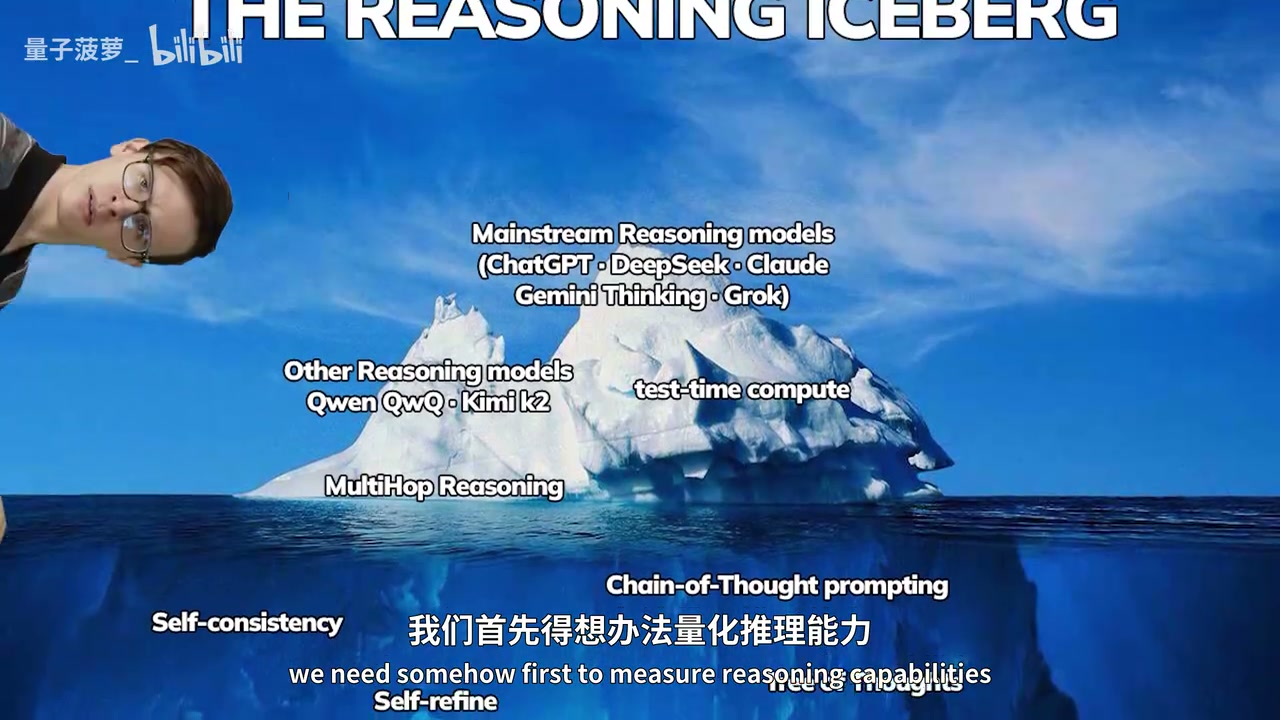
\includegraphics[width=0.82\linewidth,height=0.34\textheight,keepaspectratio]{figures/fig_01_reasoning_iceberg.jpg}
    \caption{推理能力冰山：多跳推理、测试时计算、CoT、自一致性和自我修正都在同一条“增加推理过程”的技术谱系上。\protect\footnotemark}
    \label{fig:reasoning-iceberg}
\end{figure}
\footnotetext{视频画面时间区间：00:02:29--00:02:39。}

更具体地说，测试时计算给模型提供三种机会。第一，模型可以尝试多条路径，减少一次采样失败带来的风险。第二，模型可以把复杂问题拆成较小的中间问题。第三，模型可以在后续步骤中修正前面步骤留下的粗糙表示。这里的关键词是“迭代”：没有迭代，复杂推理就会被压进一次前向计算中；有了迭代，模型至少获得了逐步改进的空间。

\subsection{多跳推理：从单步匹配到状态追踪}

多跳推理（multi-hop reasoning）是理解这件事的最小例子。视频给出的例子是：“谁是第 44 任美国总统的妻子？”这个问题需要两次跳转：先找到“第 44 任美国总统是 Barack Obama”，再找到“Barack Obama 的配偶是 Michelle Obama”。每一跳都会产生新的中间状态。

\begin{figure}[htbp]
    \centering
    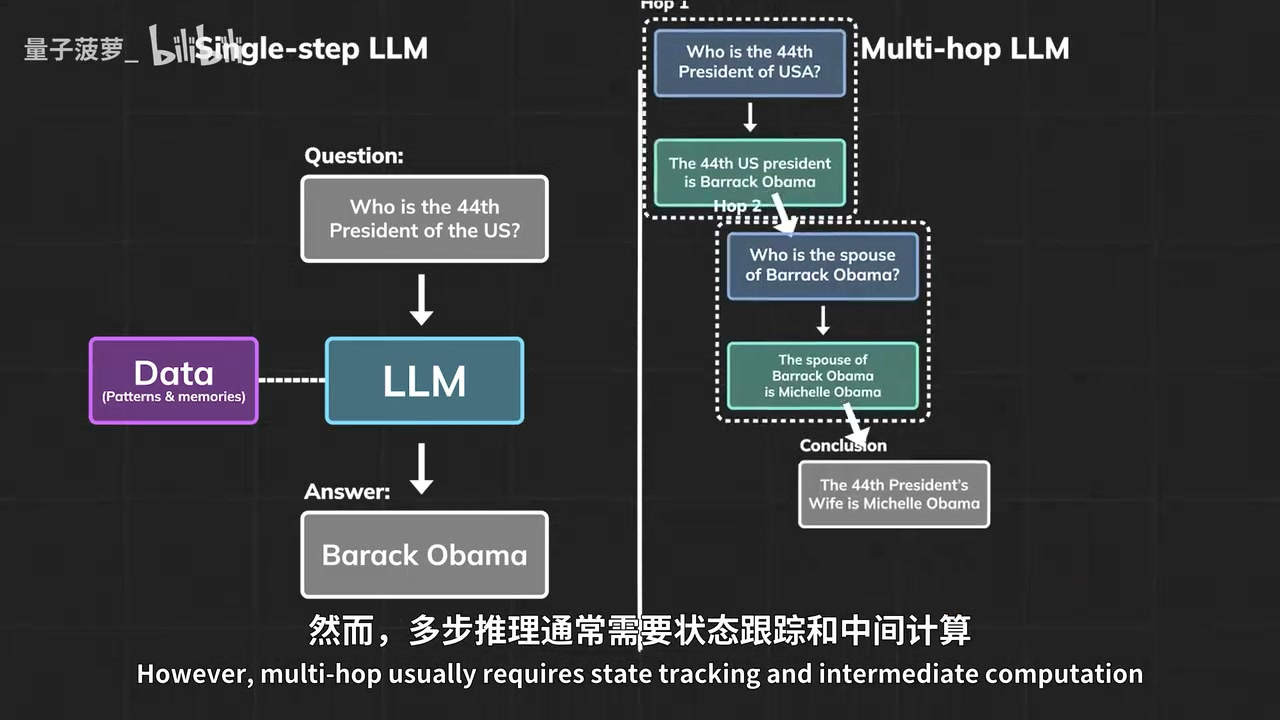
\includegraphics[width=0.82\linewidth,height=0.36\textheight,keepaspectratio]{figures/fig_02_single_vs_multihop_llm.jpg}
    \caption{单步问答更接近模式匹配；多跳推理要求模型维护中间状态，并把多个事实关系串成答案。\protect\footnotemark}
    \label{fig:single-vs-multihop}
\end{figure}
\footnotetext{视频画面时间区间：00:03:04--00:03:31。}

单步问答的难点通常是“有没有记住这个映射”。例如输入“第 44 任美国总统是谁”，输出“Barack Obama”可以近似看成从问题模式到答案模式的检索。多跳问题的难点更接近“能否保持工作记忆”。模型需要在第一跳之后保留中间答案，再把中间答案变成第二跳的查询条件。

\begin{knowledgebox}{把多跳推理想成查资料}
单步问题像在索引里查一个词条。多跳问题像先查一个词条，再把查到的结果当作第二个词条继续查。差别在于，中间结果必须被保存、引用和更新；一旦中间结果丢失，后续跳转就失去支点。
\end{knowledgebox}

这也是基础 Transformer 在多跳任务上容易吃亏的原因。若模型只能在一次生成中完成全部关系组合，它必须把所有中间计算压缩到当前隐藏表示中。跳数增加时，所需的内部计算深度也随之增加；缺少迭代机制的模型只能用参数记忆、注意力模式和一次性前向传播硬扛。

\subsection{CoT 的强处：用文本轨迹构造外部迭代}

CoT 改变了问题形态。模型先写出一个中间步骤，随后把这个中间步骤重新读回上下文，再生成下一步。这个过程让自回归模型获得了近似“循环”的效果：每一个生成的推理 token 都成为下一轮计算的输入条件。

按视频中的描述，CoT 的流程可以拆成四步：

\begin{itemize}
    \item 写出中间思考，例如先得到“第 44 任美国总统是 Barack Obama”。
    \item 回读已经写出的文本，把它并入当前上下文。
    \item 更新内部隐藏状态，让后续生成受中间结果约束。
    \item 继续写下一步，直到得到最终答案。
\end{itemize}

这解释了“多写 token 为什么能提高推理”。额外 token 承担外部状态存储的角色。文本轨迹让模型有地方放中间变量，也给训练者提供可观察的监督对象：可以筛选中间步骤，可以模仿高质量轨迹，也可以用强化学习偏好更好的推理路径。

\subsection{CoT 的代价：每次更新都穿过 token 窄门}

CoT 的笨重处也很直接：模型真正想优化的是隐藏状态中的潜在表示，实际执行时却要先把中间表示压成离散文本 token，再在下一轮把文本重新嵌入回隐藏状态。这个压缩、采样、追加上下文、再嵌入的环节让推理过程受 token 介质约束。

\begin{figure}[htbp]
    \centering
    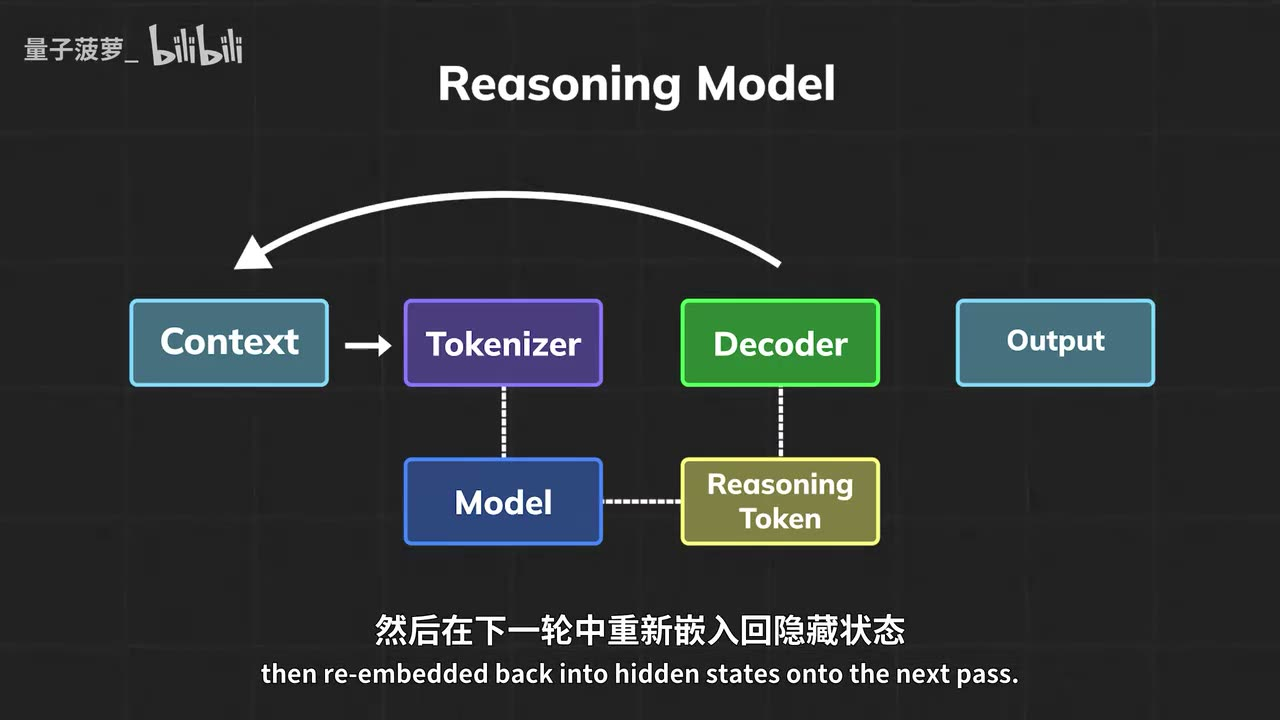
\includegraphics[width=0.82\linewidth,height=0.34\textheight,keepaspectratio]{figures/fig_03_cot_token_pipeline.jpg}
    \caption{CoT token 管线：模型把推理步骤写成 token，再把这些 token 追加到上下文并重新嵌入，形成外部化迭代。\protect\footnotemark}
    \label{fig:cot-token-pipeline}
\end{figure}
\footnotetext{视频画面时间区间：00:04:20--00:04:30。}

这张流程图给出了一条重要线索：CoT 的循环发生在文本上下文层面。模型生成 reasoning token 后，token 经过解码器形成文本输出，文本又被追加到上下文，随后重新进入 tokenizer 和模型。这个过程可以工作，甚至非常有效；代价是每一步推理都要支付离散化和上下文增长的成本。

\begin{warningbox}{常见误读}
“CoT 很重”并不等于“CoT 没价值”。它重在运行路径：中间状态要外化成 token，序列长度会增长，采样轨迹也会引入噪声。它有价值在监督路径：文本中间步骤天然可读、可筛选、可训练。后文讨论 Loop Transformer 时，这两条线需要同时记住。
\end{warningbox}

这就引出 Loop Transformer 的问题意识：如果推理的核心是反复更新隐藏状态，是否可以直接在隐藏状态中迭代？这个问题的意义超过“优雅”本身。它直接关系到计算路径、监督信号、缓存开销和部署成本。下一章会把这个直觉写成具体的循环更新机制。

\subsection{本章小结}

本章建立了后文的入口判断。第一，测试时计算提升推理的关键在于给模型更多路径和更多更新机会。第二，多跳推理把这种需求暴露得很清楚：模型必须维护中间状态，才能从一个事实跳到另一个事实。第三，CoT 通过文本 token 搭出外部迭代通道，因此有效；它同时把隐藏状态更新绑定到离散 token 管线，因此沉重。Loop Transformer 的核心动机就是把“写草稿再读回来”的外部循环，改写成隐藏状态上的内部递归。

% END INLINE section_01.tex

% BEGIN INLINE section_02.tex
\section{Loop Transformer 的核心机制：把迭代放回隐藏状态}
\label{sec:loop-transformer-core}

本章的中心判断是：Loop Transformer 把 CoT 的外部文本循环压缩为隐藏状态递归。它复用少量 Transformer 层组成共享模块，让前一次循环得到的隐藏状态成为下一次循环的输入。这样做的收益是参数更紧凑、计算过程更贴近连续表示；风险是同一模块被反复应用后，稳定性、表达能力和训练监督都会变成新问题。

\begin{importantbox}{本章主张}
Loop Transformer 的核心机制可以概括为一句话：同一个共享 Transformer 模块 \(F_\theta\) 多次作用于隐藏状态 \(h_t\)，用递归深度换取有效计算深度。
\end{importantbox}

\subsection{从 CoT 管线到隐藏状态循环}

上一章已经说明，CoT 的中间步骤要经历解码、文本追加、重新分词、重新嵌入。若把模型内部表示想成“工作记忆”，CoT 像把工作记忆的一部分写到纸上，再把纸上的文字重新读进脑中。这个类比有用，因为它点出了成本来源：真正需要更新的是隐藏表示，实际通道却绕了一圈文本。

Loop Transformer 的直觉是直接更新工作记忆。模型不必把每个中间想法先写成 token；它可以把当前隐藏状态留在连续向量空间中，并让同一个模块继续修改这份状态。视频中的“looping hidden states”画面正是在强调这个转换：推理循环从外部文本轨迹转入内部状态轨迹。

\begin{figure}[htbp]
    \centering
    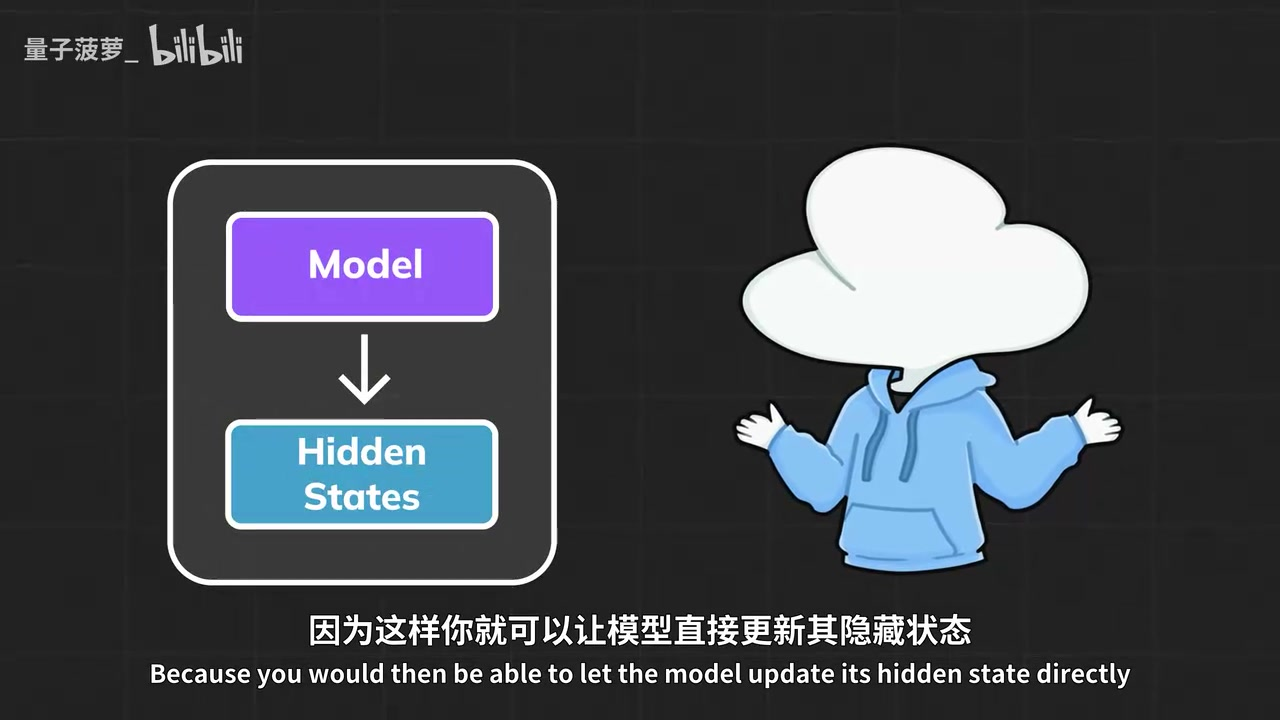
\includegraphics[width=0.82\linewidth,height=0.34\textheight,keepaspectratio]{figures/fig_04_looping_hidden_states.jpg}
    \caption{隐藏状态循环：Loop Transformer 让模型直接更新内部表示，把推理迭代放入连续状态空间。\protect\footnotemark}
    \label{fig:loop-hidden-state-update}
\end{figure}
\footnotetext{视频画面时间区间：00:04:52--00:05:04。}

\begin{knowledgebox}{类比的边界}
“脑内打磨草稿”只是帮助理解的类比。技术上，隐藏状态是高维连续向量；每次递归更新都会经过注意力、前馈网络、残差连接和归一化等操作。类比解释动机，公式和结构解释机制。
\end{knowledgebox}

\subsection{基本递归公式：同一模块反复更新状态}

先用普通话说明公式含义：循环 Transformer 把当前隐藏状态当成可更新的状态变量，把输入 \(x\) 当成问题和上下文条件，再把同一个带参数模块 \(F_\theta\) 应用到当前状态上，得到下一轮隐藏状态。多跑一次循环，就多做一次内部表示更新。

$
h_{t+1}=F_\theta(h_t,x)
$

符号说明如下：
\begin{itemize}
    \item \(h_t\)：第 \(t\) 次递归后的隐藏状态，承载模型当前的内部表示。
    \item \(h_{t+1}\)：下一次递归后的隐藏状态，也就是一次内部更新之后的新工作记忆。
    \item \(x\)：输入 token、位置、上下文或注入到循环模块中的条件信息。
    \item \(F_\theta\)：共享的 Transformer 递归模块，可以包含注意力层、前馈层和归一化结构。
    \item \(\theta\)：模块参数，在不同递归步之间共享。
    \item \(t\)：递归步编号，表示模型已经在内部循环了多少轮。
\end{itemize}

这个公式的重点在“共享”。标准深层 Transformer 可以把第 1 层、第 2 层、第 3 层分别看成不同函数；Loop Transformer 让同一个函数多次处理不断变化的状态。直观地说，参数量没有按深度线性增长，有效计算步数却可以随递归次数增长。

\subsection{残差更新：让新信息叠加到旧状态上}

实际 Transformer 中，信息通常沿残差流（residual stream）累积。残差形式的直觉是：当前状态 \(h_t\) 先保留下来，模块 \(F_\theta\) 计算一个更新量，再把旧状态和更新量相加，最后用归一化控制数值尺度。这样写可以更接近 Transformer 的信息流，也为后文稳定性章节铺路。

$
h_{t+1}=\mathrm{Norm}\bigl(h_t+F_\theta(h_t,x)\bigr)
$

符号说明如下：
\begin{itemize}
    \item \(h_t\)：进入本轮递归前的残差流状态。
    \item \(F_\theta(h_t,x)\)：共享模块根据当前状态和输入条件产生的更新量。
    \item \(h_t+F_\theta(h_t,x)\)：把旧状态与新更新叠加后的临时状态。
    \item \(\mathrm{Norm}(\cdot)\)：归一化操作，用于控制尺度并降低状态范数失控的风险。
    \item \(h_{t+1}\)：归一化之后传给下一轮递归的状态。
\end{itemize}

这条公式解释了 Loop Transformer 与普通“重复跑同一层”的区别。模型每轮沿着已有状态继续计算，并在同一条残差流上持续改写表示。状态保留了前面递归的结果，更新量则把新注意到的关系、事实或约束叠加进去。

\subsection{共享 Transformer 块：用递归深度形成有效深度}

视频中展示的 recurrent Transformer block 把机制画得更具体：一个包含多头注意力（Multi-Head Attention）和前馈网络（Feed-Forward）的块被环形箭头包住，表示输出会回到同一块中继续处理。前一次循环的输出隐藏状态成为下一次循环的输入，这正是“循环”一词的结构含义。

\begin{figure}[htbp]
    \centering
    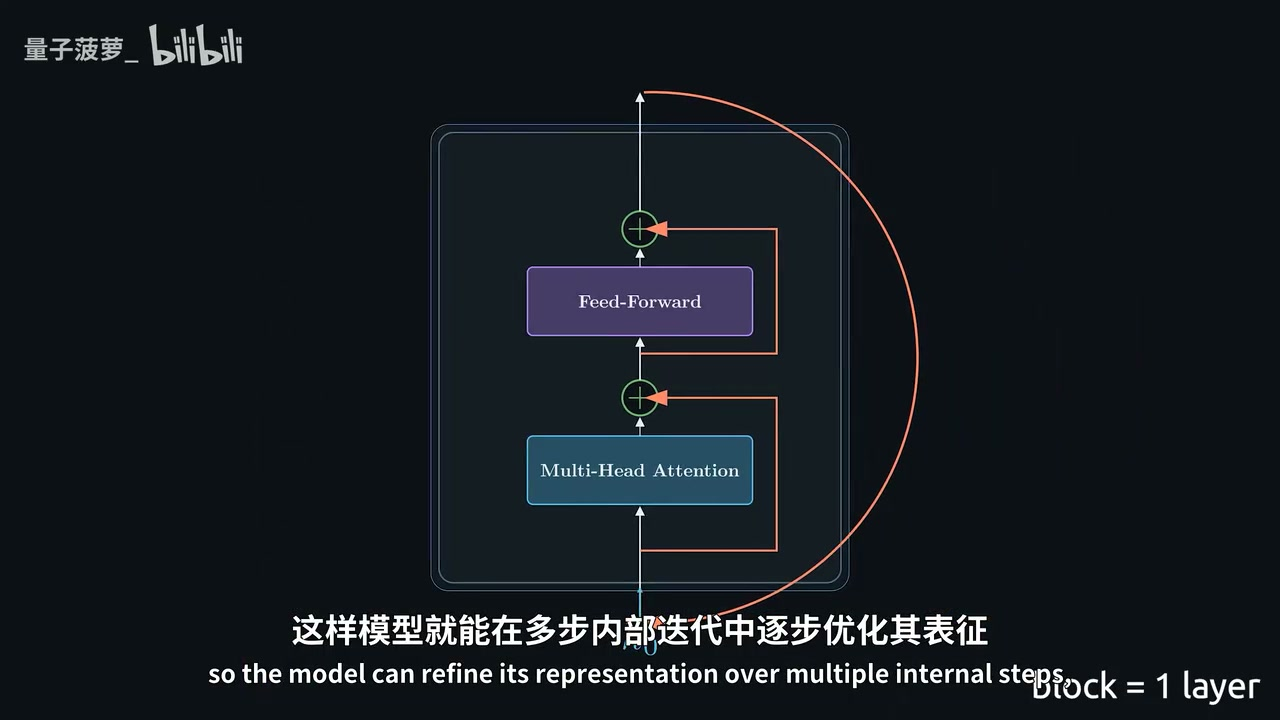
\includegraphics[width=0.82\linewidth,height=0.36\textheight,keepaspectratio]{figures/fig_05_recurrent_transformer_block.jpg}
    \caption{共享 Transformer 块反复作用于残差流，让模型在多步内部递归中逐步打磨表示。\protect\footnotemark}
    \label{fig:recurrent-transformer-block}
\end{figure}
\footnotetext{视频画面时间区间：00:05:25--00:05:40。}

这里有一个容易被忽略的点：共享权重并不自动意味着每一步功能相同。原因在于输入状态已经改变。同一个函数 \(F_\theta\) 处理 \(h_0\)、\(h_1\)、\(h_2\) 时，看到的是不同状态，因此可以表现出阶段化行为：早期整理问题，中期整合关系，后期收敛答案。第三章会把这个判断和行为证据连起来。

\begin{warningbox}{机制边界}
Loop Transformer 的“有效深度”来自重复应用共享模块。它能节省参数，也能提供更多内部更新机会；它同样带来约束，因为每一步都受同一组参数控制。后续章节需要继续检查：这种约束是否稳定、是否可外推、是否真的形成可复用推理过程。
\end{warningbox}

\subsection{本章小结}

本章把 Loop Transformer 的核心机制压缩成两条公式和一个结构图。基本公式 \(h_{t+1}=F_\theta(h_t,x)\) 表示同一共享模块递归更新隐藏状态；残差公式 \(h_{t+1}=\mathrm{Norm}(h_t+F_\theta(h_t,x))\) 表示更新沿残差流叠加并受归一化控制。这个设计把 CoT 的外部 token 循环转入内部状态循环，用递归深度换取有效计算深度。下一章要回答更关键的问题：这种内部递归是否带来了可观察的行为收益。

% END INLINE section_02.tex

% BEGIN INLINE section_03.tex
\section{证据一：多跳外推与三阶段泛化}
\label{sec:grokking-evidence}

本章的结论是：视频给出的多跳外推和三阶段泛化证据，说明递归深度可能形成可复用的计算过程。这个证据有技术价值，也需要严格限界。它支持“循环次数可以成为测试时计算旋钮”这一判断；它尚不足以推出循环 Transformer 已经拥有通用推理优势。

\begin{importantbox}{本章主张}
行为证据的核心意义在于：当推理时增加循环次数，模型有机会处理比训练阶段更长的关系链。若这种外推稳定出现，递归模块除节省参数外，还可能学到可重复调用的推理更新规则。
\end{importantbox}

\subsection{《Loop, Think, and Generalize》的证据入口}

视频在 00:05:40 之后提到《Loop, Think, and Generalize》，并把它作为 Loop Transformer 行为证据的入口。讲义应把这里写成“视频中的论文叙述”：循环架构在多跳推理任务上表现更好，并且当推理阶段增加循环迭代时，模型能够处理超过训练深度的跳数。

这个现象如果成立，含义很重要。模型训练时只见过较短的跳数，推理时却能通过更多循环处理更长链条，说明它可能学到了一种“重复应用的关系更新规则”。类比到查资料：训练时只练过“查两次索引”，测试时增加循环次数后可以查三次、四次；关键能力在于每次查到中间结果后，仍能把它转成下一次查询的有效状态。

\subsection{三阶段 Grokking：从记忆到系统化组合}

视频画面中的三阶段顿悟式泛化（grokking）曲线把训练过程分成三个阶段：记忆训练样本、分布内泛化、系统化泛化。它的教学价值在于让读者看到，模型能力提升可能呈现阶梯式打开，偏离“平滑多记一点”的朴素想象。

\begin{figure}[htbp]
    \centering
    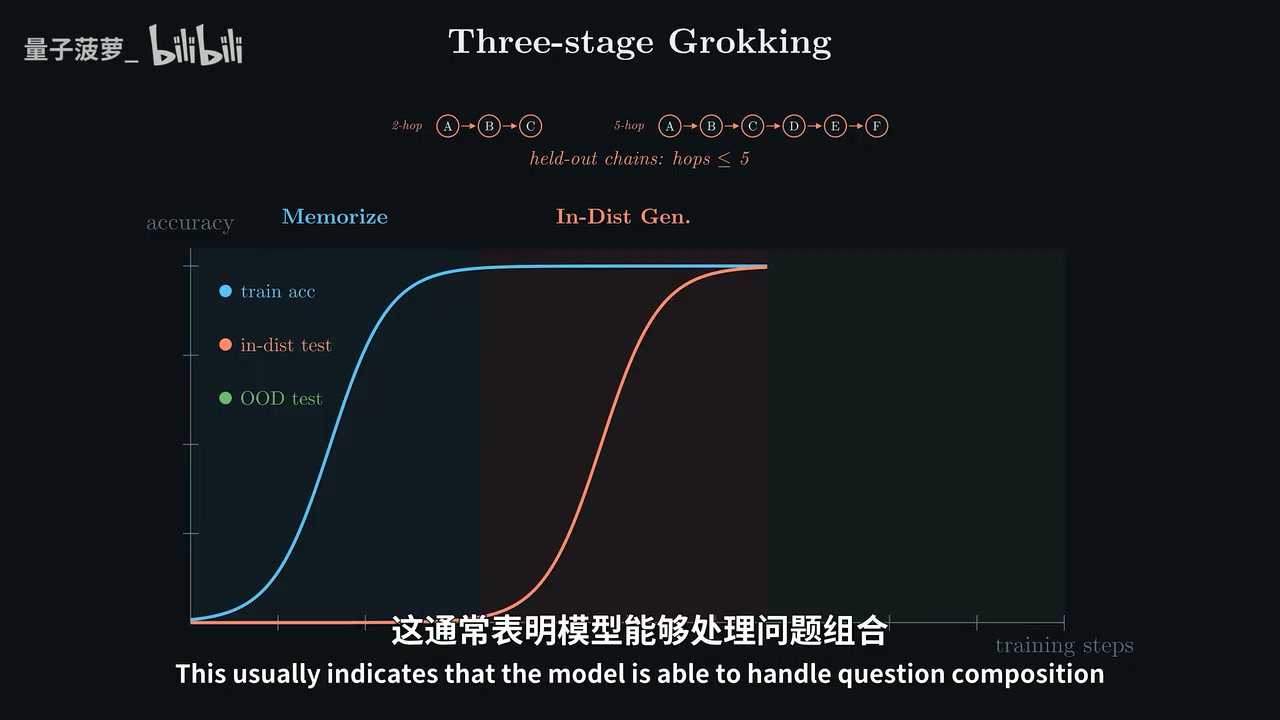
\includegraphics[width=0.82\linewidth,height=0.36\textheight,keepaspectratio]{figures/fig_06_three_stage_grokking.jpg}
    \caption{三阶段 grokking 曲线：训练准确率先上升，随后分布内测试提升，最后才出现面向未见组合的系统化泛化。\protect\footnotemark}
    \label{fig:grokking-three-stages}
\end{figure}
\footnotetext{视频画面时间区间：00:06:00--00:06:24。}

第一阶段是记忆（memorization）。蓝色训练准确率先上升，表示模型逐渐掌握训练样本中的具体链条。这个阶段像背题：给定熟悉组合，模型能够答对。

第二阶段是分布内泛化（in-distribution generalization）。橙色测试曲线随后上升，表示模型开始处理与训练结构相同、具体样本不同的问题。这个阶段像学会同一类题的解法：题目换了，规则仍相近。

第三阶段是系统化泛化（systematic generalization）。视频把它描述为模型能够组合训练期间未组合过的知识片段，也就是对分布外（out-of-distribution, OOD）组合的处理能力增强。这个阶段最接近“学会规则”：模型不只复述见过的路径，还能把局部关系重新拼接成新的答案链。

\begin{knowledgebox}{为什么 grokking 容易被误读}
Grokking 常被理解为“模型突然开窍”。更严格的说法是：不同评测集合上的准确率在训练过程中先后跨过阈值。它展示的是行为曲线的阶段性变化；若要证明内部算法，还需要后续的机制分析，例如隐藏状态轨迹、固定点、注意力头行为等证据。
\end{knowledgebox}

\subsection{递归深度作为测试时计算旋钮}

视频在 00:06:47 之后强调：当推理时增加循环次数，模型可以完成比训练时更多的跳跃。在 Loop Transformer 中，递归次数 \(R\) 就成为一种计算调节器。普通 CoT 通过生成更多 token 增加计算；循环模型通过增加内部递归步增加计算。

先用普通话解释这个公式：若训练时模型主要使用 \(R_{\mathrm{train}}\) 次循环，推理时把循环次数提高到 \(R_{\mathrm{test}}\)，模型就在更长的状态更新链上应用同一个规则。计算量会随递归次数增加而增加，收益取决于这个更新规则是否能稳定外推。

$
R_{\mathrm{test}}>R_{\mathrm{train}},\qquad C_{\mathrm{loop}}\propto R_{\mathrm{test}}
$

符号说明如下：
\begin{itemize}
    \item \(R_{\mathrm{train}}\)：训练阶段使用或主要暴露给模型的递归次数。
    \item \(R_{\mathrm{test}}\)：推理阶段实际运行的递归次数。
    \item \(C_{\mathrm{loop}}\)：循环推理的近似计算成本。
    \item \(\propto\)：正比关系，用于表达“递归次数越多，计算成本越高”的一阶直觉。
\end{itemize}

这个公式的价值在于把“更长时间思考”落到可调参数上。CoT 的旋钮是 token 数和采样路径；Loop Transformer 的旋钮是递归深度。两者都属于测试时计算，只是一个发生在文本序列中，一个发生在隐藏状态中。

\subsection{证据边界：有力线索与过度外推之间}

本章必须谨慎。多跳表现提升和超过训练深度的外推，是支持循环架构的有力线索；它们还只能说明“递归深度可能形成可复用计算过程”。若把它直接写成“循环 Transformer 已经证明通用推理能力更强”，证据链会过长。

\begin{warningbox}{证据边界}
受控多跳任务能检验关系链追踪、状态保持和组合泛化。真实大规模推理还包含噪声上下文、开放世界知识、工具调用、长程依赖、训练分布偏差和系统延迟约束。三阶段曲线说明了值得继续研究的方向，尚需和机制分析、稳定性、缓存成本以及真实任务评测共同判断。
\end{warningbox}

因此，本章与第二章之间的关系应当这样理解：第二章定义了递归机制，第三章说明这种机制可能带来行为收益。后续章节还需要回答两个硬问题：重复应用同一模块是否稳定，以及隐藏状态里发生的变化是否可观察、可解释、可监督。

\subsection{本章小结}

本章从视频中的《Loop, Think, and Generalize》叙述出发，解释了三阶段 grokking 与多跳外推的意义。记忆阶段说明模型先掌握训练样本；分布内泛化说明模型开始处理同结构新题；系统化泛化说明模型可能学到可组合的关系更新规则。递归深度 \(R\) 因此成为测试时计算旋钮：增加循环次数可以给模型更多内部更新机会。结论需要克制：这些行为证据支持“递归可能学到可复用计算过程”，后文仍需检查稳定性、机制可解释性和工程边界。

% END INLINE section_03.tex

% BEGIN INLINE section_04.tex
\section{稳定性：循环模型首先是一个动态系统}
\label{sec:stability-dynamical-system}

本章的核心判断是：循环 Transformer（Loop Transformer）一旦把同一个共享模块反复作用在隐藏状态上，它就已经进入动态系统（dynamical system）问题域。性能能否随着递归深度增加而改善，先取决于状态轨迹能否保持可控；如果残差流（residual stream）里的隐藏状态范数失控，后续所有“内部思考”的解释都会失去基础。

\begin{importantbox}{本章主张}
循环模型的第一道硬门槛是稳定性。递归深度带来额外计算，也带来误差放大、状态偏移和损失脉冲；约束与归一化的作用，是让每次更新都在可控范围内推进。
\end{importantbox}

\subsection{从递归深度到动态系统}

前一章把递归深度解释成测试时计算的调节器：模型可以在推理时多运行几轮共享块，让隐藏状态获得更多更新机会。本章要补上一层更底层的事实：同一个函数被重复调用时，微小偏差会沿着递归链条传播。若每一步都把状态推离稳定区域，循环次数越多，模型越容易把可用表示放大成噪声。

视频在 00:07:03--00:07:40 强调了这个问题：循环架构从一串彼此独立的层，转为对隐藏状态重复应用相同变换；此时需要决定循环次数，并确保信息不会在反复更新中变得混乱。直观类比是反复调整同一份草稿：每次修改都可能让表达更清楚，也可能把前一步的小误差扩成整段文字的偏题。模型内部也类似，只是草稿从文本变成了连续向量。

先用朴素语言说公式要表达的内容：隐藏状态 \(h_t\) 是第 \(t\) 次递归后的内部表示；下一轮状态由旧状态经过同一个更新规则得到，同时混入输入信息。画面中的简化形式把复杂的 Transformer 更新线性化为两部分：旧状态的传播和输入的注入。

\[
h_{t+1}=Ah_t+Bx
\]

符号说明：
\begin{itemize}
  \item \(h_t\)：第 \(t\) 次递归后的隐藏状态，也就是模型当前的内部工作记忆。
  \item \(h_{t+1}\)：下一次递归后的隐藏状态。
  \item \(A\)：旧隐藏状态如何被继续传播和变换的简化矩阵。
  \item \(B\)：输入 \(x\) 如何被注入当前状态的简化矩阵。
  \item \(x\)：当前 token 或上下文输入提供的信息。
\end{itemize}

这个式子只是讲义层面的线性化直觉。真实的 Transformer 块包含 attention、MLP、归一化和残差连接，通常可以写成更一般的共享更新：

\[
h_{t+1}=F_\theta(h_t,x)
\]

符号说明：
\begin{itemize}
  \item \(F_\theta\)：被反复复用的 Transformer 递归模块，\(\theta\) 是共享参数。
  \item \(h_t\)：递归前的隐藏状态。
  \item \(x\)：输入信息或注入到循环中的上下文表示。
  \item \(h_{t+1}\)：应用同一模块后得到的新状态。
\end{itemize}

\begin{figure}[htbp]
  \centering
  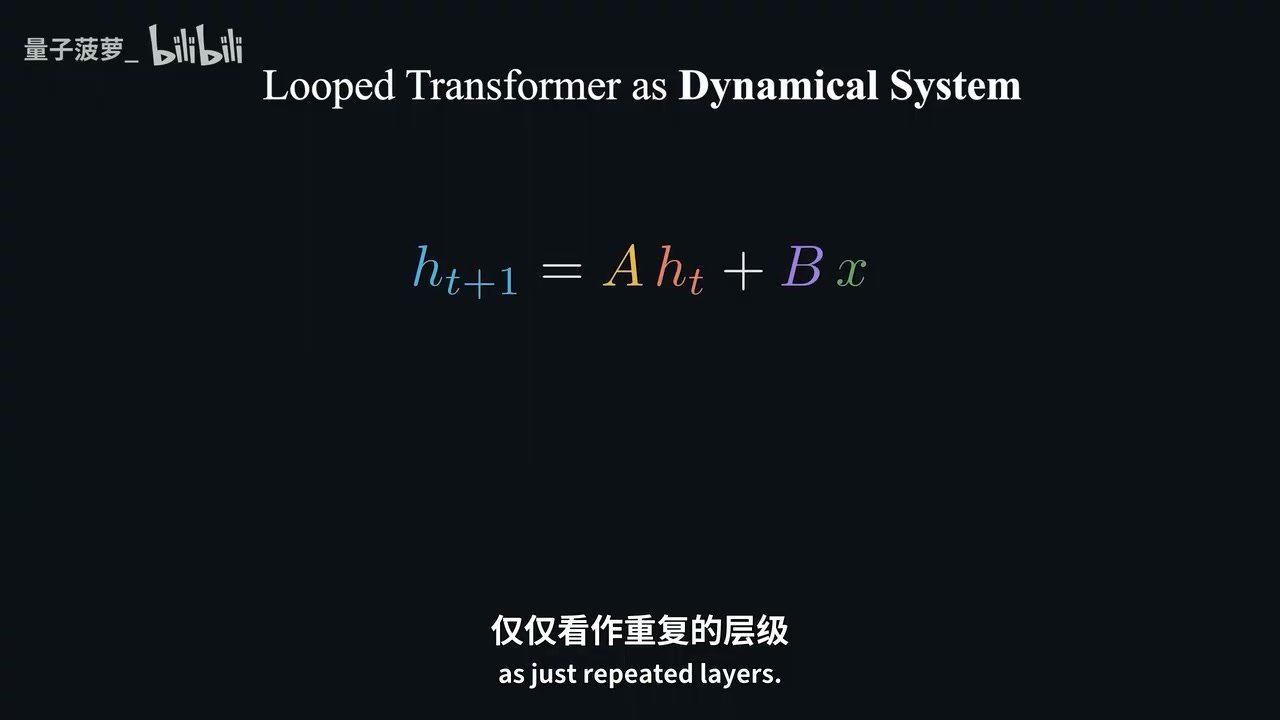
\includegraphics[width=0.82\linewidth,height=0.36\textheight,keepaspectratio]{figures/fig_07_dynamical_system_equation.jpg}
  \caption{循环 Transformer 被视为动态系统后，隐藏状态更新可以用 \(h_{t+1}=Ah_t+Bx\) 这样的简化形式建立直觉。\protect\footnotemark}
  \label{fig:residual-stream-dynamics}
\end{figure}
\footnotetext{视频画面时间区间：00:07:43--00:07:52。}

\subsection{残差流为什么成为状态主通道}

动态系统视角之所以落在残差流上，是因为残差流承载了 Transformer 层间持续传递的信息。标准深层 Transformer 中，每一层都有自己的参数，残差流像一条主干河道，沿途接受不同支流的注入。循环 Transformer 中，主干河道依旧存在，只是同一套处理装置被反复接到河道上；每一轮都读取旧状态、混入输入、执行 Transformer 操作，再把结果写回残差流。

视频在 00:07:52--00:08:15 说明了这个机制：隐藏状态每次出现都会向前传播并更新，而非从头重新计算；每次循环都会重用之前的隐藏状态，并与注入输入混合。因此，残差流本质上就是递归过程里的潜在状态（latent state）。如果这个通道有序，递归可以逐步整合信息；如果这个通道失控，递归只会把混乱带到下一轮。

为了说明稳定更新，讲义可以把残差更新写成“旧状态加上本轮修正，再做归一化”。这条公式表达的是：循环块不应每轮重造一个全新状态，而应在旧状态上追加受控修正。

\[
h_{t+1}=\mathrm{Norm}\bigl(h_t+\Delta_\theta(h_t,x)\bigr)
\]

符号说明：
\begin{itemize}
  \item \(h_t\)：进入第 \(t+1\) 次递归前的残差流状态。
  \item \(\Delta_\theta(h_t,x)\)：共享模块根据当前状态和输入产生的本轮修正量。
  \item \(h_t+\Delta_\theta(h_t,x)\)：残差式累积，表示旧状态被保留并被更新。
  \item \(\mathrm{Norm}(\cdot)\)：归一化或约束操作，用来限制尺度漂移。
  \item \(h_{t+1}\)：归一化后的下一轮状态。
\end{itemize}

\begin{knowledgebox}{稳定性直觉}
从第一性原理看，循环模型的危险来自“反复乘上同一个变化”。若某个方向上的更新每轮都会把向量长度放大 \(1.1\) 倍，十几轮后就会形成明显漂移；若更新被约束在稳定范围内，递归才可能像迭代求解器一样逐步逼近有用表示。
\end{knowledgebox}

\subsection{隐藏状态范数、损失脉冲与发散}

稳定性最容易观察的信号之一是隐藏状态范数（hidden-state norm）。范数可以理解为向量“有多大”：它不直接告诉读者状态里的语义是否正确，却能提醒读者状态尺度是否正在失控。视频在 00:08:15--00:08:27 指出：如果动态系统不稳定，隐藏状态的范数会在递归中增长，引发训练损失（training loss）的脉冲和发散；约束与归一化的任务，就是防止每次更新因为不受控累积而崩溃。

先用白话解释下面的量：若模型每轮更新都让 \(\lVert h_t\rVert\) 变大，训练损失 \(L_t\) 往往会出现突增。这个突增并不神秘，它常常意味着模型内部状态进入了训练过程很难处理的尺度范围。

\[
\lVert h_{t+1}\rVert \le \alpha \lVert h_t\rVert+\beta \lVert x\rVert,\qquad 0\le \alpha \lesssim 1
\]

符号说明：
\begin{itemize}
  \item \(\lVert h_t\rVert\)：第 \(t\) 次递归后隐藏状态的范数，表示状态尺度。
  \item \(\lVert h_{t+1}\rVert\)：下一轮状态尺度。
  \item \(\alpha\)：旧状态在下一轮中被放大的程度；接近或低于 \(1\) 更利于稳定。
  \item \(\beta\)：输入信息对状态尺度的影响强度。
  \item \(\lVert x\rVert\)：输入表示的范数。
\end{itemize}

这里的关键是稳定性约束的方向：旧状态的影响不能无限放大，输入注入也要有边界。对工程实现来说，这通常会落到 normalization、residual scaling、门控、训练初始化和递归步数策略上。

\begin{figure}[htbp]
  \centering
  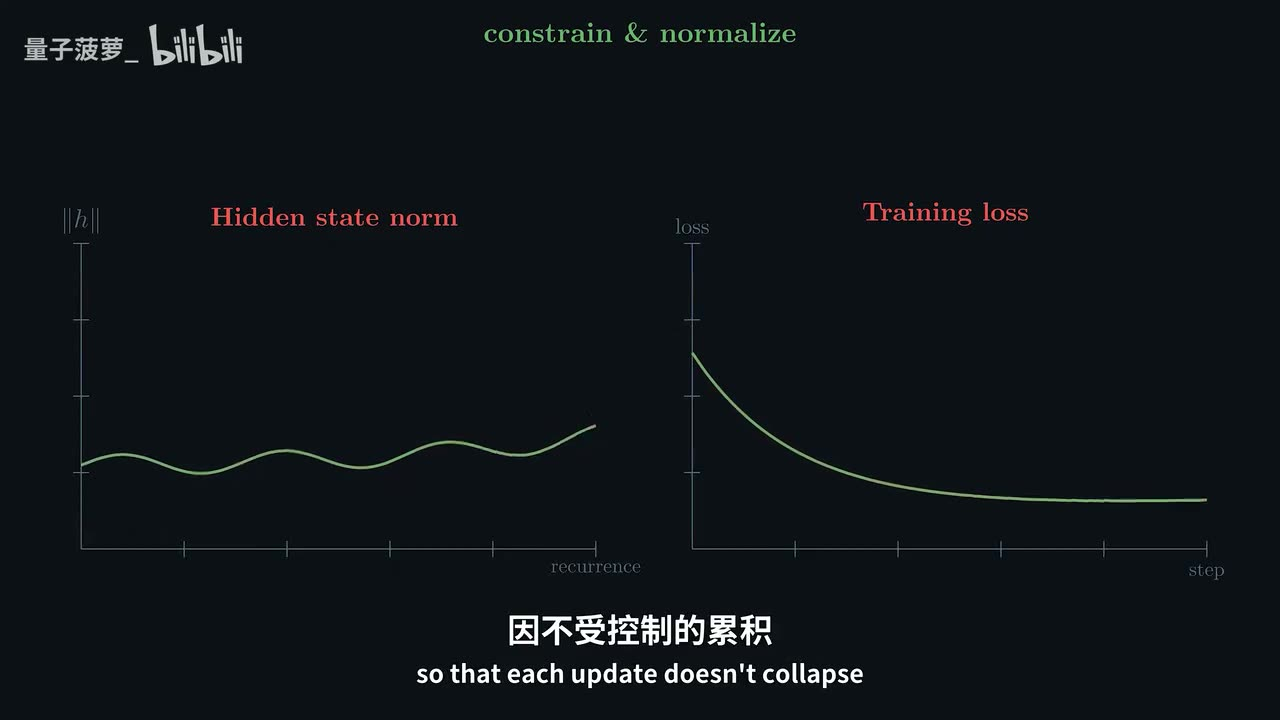
\includegraphics[width=0.82\linewidth,height=0.36\textheight,keepaspectratio]{figures/fig_08_instability_norm_loss.jpg}
  \caption{约束与归一化用于限制隐藏状态范数的失控增长，从而减少训练损失中的脉冲和发散风险。\protect\footnotemark}
  \label{fig:instability-norm-loss}
\end{figure}
\footnotetext{视频画面时间区间：00:08:20--00:08:30。}

\subsection{固定点和周期：下一章证据的预备概念}

一旦把循环模型看成动态系统，读者自然会问：反复更新最后会去哪里？有三种典型结局。第一种是趋近固定点（fixed point），状态越来越接近某个稳定位置；第二种是进入周期轨迹（cycle），状态在若干个区域之间有规律地来回访问；第三种是发散，状态尺度或方向不断失控。前两种至少说明系统存在结构，第三种通常意味着模型难以可靠使用。

固定点的直觉是：再更新一轮，状态也几乎不变。

\[
h^\star \approx F_\theta(h^\star,x)
\]

符号说明：
\begin{itemize}
  \item \(h^\star\)：递归过程趋近的稳定隐藏状态。
  \item \(F_\theta\)：共享递归模块。
  \item \(x\)：输入或上下文信息。
  \item \(\approx\)：表示近似相等，实际模型中通常只能观察到接近稳定。
\end{itemize}

周期轨迹的直觉是：状态隔 \(p\) 轮后回到相似区域。

\[
h_{t+p}\approx h_t
\]

符号说明：
\begin{itemize}
  \item \(t\)：当前递归步。
  \item \(p\)：周期长度，表示经过多少轮后回到相似状态。
  \item \(h_{t+p}\)：第 \(t+p\) 次递归后的状态。
  \item \(h_t\)：第 \(t\) 次递归后的状态。
\end{itemize}

\begin{warningbox}{稳定性证据边界}
稳定轨迹只说明递归过程没有明显乱跑或崩溃。它还不能直接证明模型学会了人类可解释的推理算法。下一章的机制证据必须继续追问：这些轨迹是否和注意力行为、推理阶段、答案收敛相互呼应。
\end{warningbox}

\subsection{本章小结}

本章把 Loop Transformer 从“重复运行几层”推进到“在残差流上定义动态系统”。读者应带走三个判断：第一，递归深度带来计算机会，也放大稳定性风险；第二，残差流是隐藏状态前后传递的主通道，归一化和约束是在保护这条通道；第三，固定点和周期轨迹是观察内部递归结构的入口，真正的机制解释还需要结合下一章的 PCA、注意力稳定和阶段化递归证据。

% END INLINE section_04.tex

% BEGIN INLINE section_05.tex
\section{证据二：隐藏状态轨迹、固定点、周期与推理阶段}
\label{sec:mechanistic-analysis}

本章的核心判断是：多跳性能提升只能说明循环深度可能有用，机制分析才开始回答“模型内部是否形成了有结构的递归过程”。视频给出的证据链是：追踪隐藏状态，用主成分分析（Principal Component Analysis, PCA）投影到低维空间，观察固定点与周期轨迹，再检查注意力行为和早期、中期、后期递归阶段是否出现稳定分工。

\begin{importantbox}{本章主张}
权重共享不等于每一步执行同样的功能。输入到共享块的隐藏状态每轮都不同，同一个函数会在不同递归阶段呈现不同作用：早期形成粗表示，中期整合关系，后期稳定并收敛到答案。
\end{importantbox}

\subsection{为什么性能证据还不够}

视频在 00:08:31--00:08:49 明确提出了一个必要怀疑：即使模型多跳表现更好，也不能只凭结果断言它“真的在推理”。一个模型可能因为数据分布、任务模板、训练捷径而表现提升；要建立更强判断，需要看递归过程内部是否有可观察结构。

这里的第一性原理很直接：若循环模型只是把隐藏状态随机扰动几次，性能偶然提升的解释就很脆弱；若隐藏状态沿着稳定轨迹移动，且注意力行为也随之稳定，读者才有理由相信递归步骤在执行某种一致的计算。机制证据并不会把模型彻底解释清楚，它能排除一部分“只是乱动”的解释。

\subsection{PCA：把高维递归轨迹压到可观察平面}

隐藏状态通常有几千甚至上万维，人眼无法直接观察。PCA 的作用是找出激活变化最大的几个方向，把高维状态投影到二维或三维平面。这样读者可以看到递归轨迹是向某个区域收敛、围绕某个轨道运动，还是快速散开。

先用白话解释下面的公式：PCA 会从一批隐藏状态里估计平均状态 \(\mu\)，再取最能解释变化的主方向 \(W_k\)。每个高维状态 \(h_t\) 被减去均值后投影到这些主方向上，得到低维坐标 \(z_t\)。

\[
z_t=W_k^\top(h_t-\mu),\qquad k\in\{2,3\}
\]

符号说明：
\begin{itemize}
  \item \(h_t\)：第 \(t\) 次递归后的高维隐藏状态。
  \item \(\mu\)：用于居中的平均隐藏状态。
  \item \(W_k\)：前 \(k\) 个主成分方向组成的矩阵。
  \item \(z_t\)：低维投影坐标，用于画出递归轨迹。
  \item \(k\)：投影维度，常取 \(2\) 或 \(3\)，便于可视化。
\end{itemize}

\begin{knowledgebox}{PCA 的作用边界}
PCA 像给高维房间装一盏投影灯：它能把主要运动方向投到墙上，让人看见轨迹形状。代价也很清楚，墙上的影子会丢掉一部分维度信息，所以 PCA 图适合提示结构，不能单独充当完整证明。
\end{knowledgebox}

\subsection{固定点与周期：递归过程趋向稳定结构}

视频在 00:09:20--00:09:43 说明，机制分析观察到循环模型在潜在空间中趋向稳定轨迹：一些情况像固定点，表示表征逐渐稳定；另一些情况呈现周期轨迹，隐藏状态在重复块中访问一致状态。这说明内部状态没有不可预测地快速坍缩，也没有无界漂移。

固定点表达的是“更新后几乎仍在原处”。在推理语境里，它可以理解为模型已经把相关信息整合到一个稳定表示中，继续递归带来的变化变小。

\[
h^\star \approx F_\theta(h^\star,x)
\]

符号说明：
\begin{itemize}
  \item \(h^\star\)：稳定隐藏状态或近似收敛点。
  \item \(F_\theta\)：共享递归模块。
  \item \(x\)：输入或上下文。
  \item \(\approx\)：近似相等，表示实际观测中存在小幅更新。
\end{itemize}

周期轨迹表达的是“隔若干轮回到相似位置”。它不代表模型没有进展，可能代表系统在几个互补状态之间有规律切换，例如反复在候选关系和答案表示之间调整。

\[
h_{t+p}\approx h_t,\qquad p\ge 2
\]

符号说明：
\begin{itemize}
  \item \(h_t\)：第 \(t\) 次递归后的状态。
  \item \(h_{t+p}\)：经过 \(p\) 轮后的状态。
  \item \(p\)：周期长度。
  \item \(\approx\)：表示两个状态在低维投影或相似性度量上接近。
\end{itemize}

\begin{figure}[htbp]
  \centering
  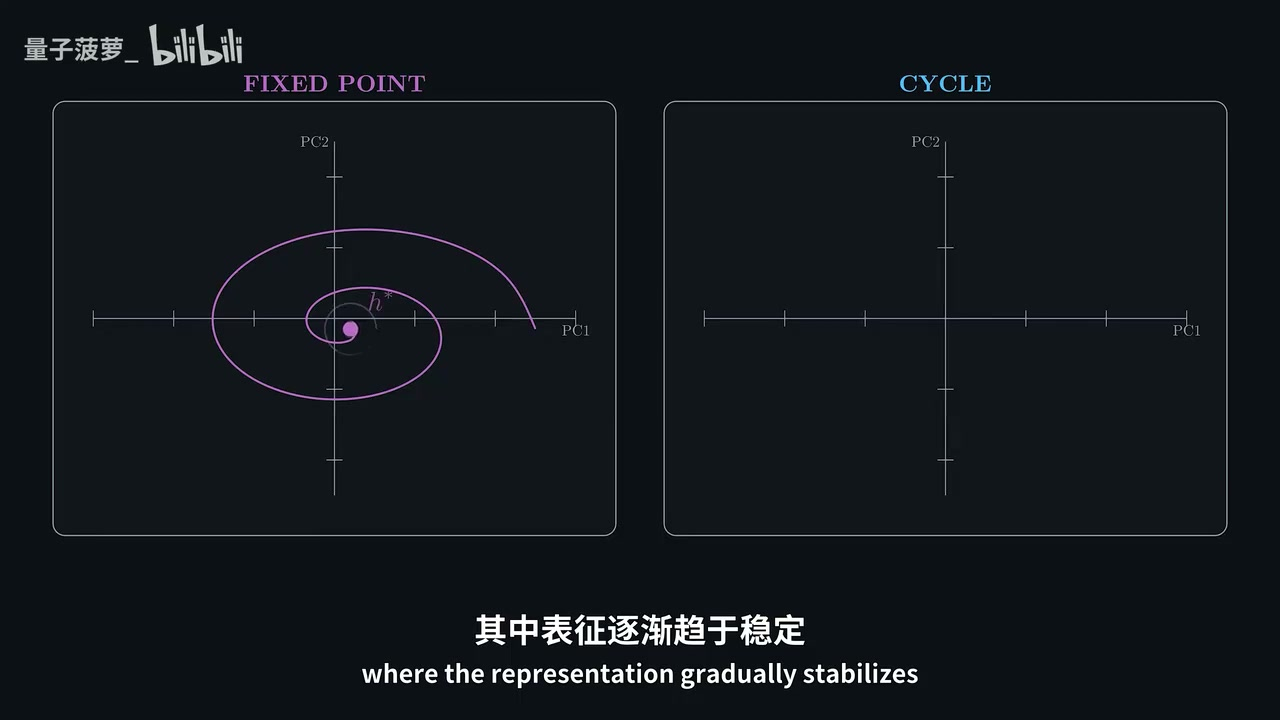
\includegraphics[width=0.82\linewidth,height=0.36\textheight,keepaspectratio]{figures/fig_09_fixed_point_cycle.jpg}
  \caption{PCA 视角下的固定点与周期轨迹：前者显示状态逐步稳定，后者显示状态在一致区域之间有规律往复。\protect\footnotemark}
  \label{fig:pca-fixed-point-cycle}
\end{figure}
\footnotetext{视频画面时间区间：00:09:20--00:09:37。}

\subsection{注意力稳定：状态稳定还要对应计算稳定}

只看激活轨迹仍然不够。隐藏状态稳定可能只是数值上变得平滑，未必意味着模型正在执行一致计算。视频在 00:09:43--00:10:00 补了第二层证据：当隐藏状态接近固定点或周期轨迹时，注意力头（attention head）的行为也趋于稳定；这意味着块内部执行的计算也更一致。

这个点很关键。attention 决定了 token 之间如何交换信息。若隐藏状态轨迹趋稳，同时 attention 模式也趋稳，那么递归过程更像一个逐步收敛的计算程序；若两者分离，PCA 图就可能只是漂亮的几何图案。讲义需要把这一层边界讲清楚：机制证据的强度来自多种观测相互支持，而非单张 PCA 图。

\begin{warningbox}{机制证据边界}
PCA 图不能直接证明“模型学会了人类可解释的推理算法”。它能显示轨迹形状，注意力分析能补充计算行为是否稳定；二者合在一起，才构成比性能曲线更强的机制线索。
\end{warningbox}

\subsection{早期、中期、后期：共享块如何形成阶段化功能}

视频在 00:10:02--00:11:00 给出了本章最有教学价值的观察：同一共享块在递归过程的不同阶段承担不同角色。早期递归构建问题的粗略表示，收集并组织相关信息，更新幅度更大也更具探索性；中期递归开始整合信息并传递关系，更新更结构化；后期递归主要稳定表示并收敛到最终答案。

这件事听起来反直觉，因为共享权重意味着每轮调用的是同一个函数。关键在于函数的输入已经变了。可把共享块想成同一位编辑：第一遍拿到的是混乱草稿，所以任务是搭框架；第二遍看到的是已有结构的稿件，所以任务变成补关系；最后一遍面对接近完成的稿件，任务转为收敛和校正。同一位编辑，面对不同阶段的文本，会做出不同动作。

\begin{figure}[htbp]
  \centering
  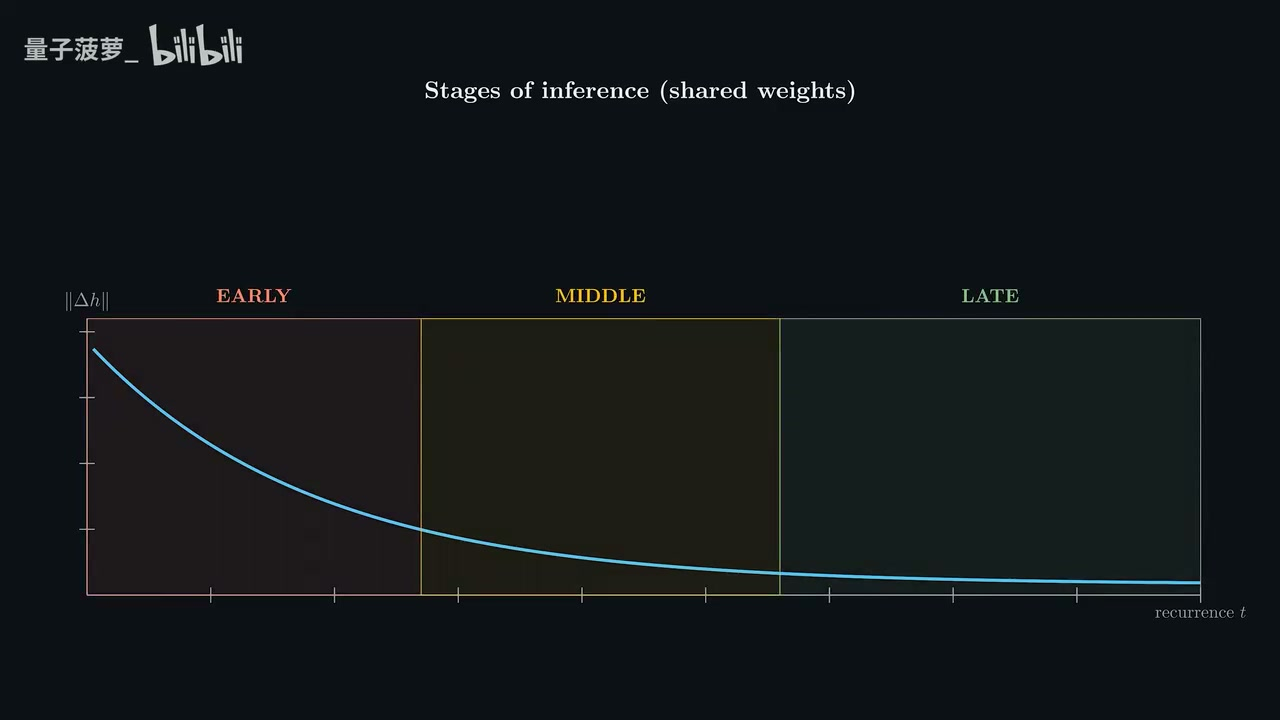
\includegraphics[width=0.82\linewidth,height=0.36\textheight,keepaspectratio]{figures/fig_10_stages_of_inference.jpg}
  \caption{共享权重下的推理阶段：早期更新幅度大，中期逐步结构化，后期趋于稳定和收敛。\protect\footnotemark}
  \label{fig:stages-of-inference}
\end{figure}
\footnotetext{视频画面时间区间：00:10:02--00:10:45。}

可以用一个简单的更新差分表达阶段变化。它先说明每一轮状态变化有多大，再把“早期大、中期结构化、后期变小”落到数学对象上。

\[
\Delta_t=h_{t+1}-h_t,\qquad \lVert \Delta_{\mathrm{early}}\rVert>\lVert \Delta_{\mathrm{late}}\rVert
\]

符号说明：
\begin{itemize}
  \item \(\Delta_t\)：第 \(t\) 次递归带来的状态变化。
  \item \(h_t\)：第 \(t\) 次递归后的隐藏状态。
  \item \(h_{t+1}\)：下一轮隐藏状态。
  \item \(\lVert \Delta_{\mathrm{early}}\rVert\)：早期递归更新幅度。
  \item \(\lVert \Delta_{\mathrm{late}}\rVert\)：后期递归更新幅度。
\end{itemize}

这个式子不声称所有模型都必须满足严格单调下降。它只是在讲义中表达视频所说的阶段化直觉：早期更像探索，中期更像关系整合，后期更像稳定答案。

\subsection{本章小结}

本章把“递归可能增强推理”的说法推进到机制层面。读者应带走四点：第一，性能提升需要内部轨迹证据支持；第二，PCA 能把高维状态投影成可观察轨迹，也会丢失信息；第三，固定点、周期和注意力稳定共同提示递归过程具有结构；第四，共享权重仍可形成阶段化功能，因为每一轮输入到共享块的状态已经不同。下一章将沿着这个逻辑追问计算效率：既然所有 token 固定递归会浪费计算，MoR 如何让不同 token 使用不同递归深度。

% END INLINE section_05.tex

% BEGIN INLINE section_06.tex
\section{MoR：让不同 token 使用不同递归深度}
\label{sec:mixture-of-recursions}

本章的核心判断是：固定递归步数把所有 token 当成同样困难的问题处理，计算上很粗糙。混合递归（Mixture-of-Recursions, MoR）的目标，是让简单 token 提前结束，让复杂 token 获得更多内部更新；它把“递归深度”从全局超参数变成 token 级别的路由决策。

\begin{importantbox}{本章主张}
MoR 的关键收益来自计算分配，而非凭空减少推理难度。路由器（router）负责判断每个 token 需要多少递归；判断越早，执行越规整；判断越晚，适应性越强，训练和稳定性也更麻烦。
\end{importantbox}

\subsection{固定递归的低效性}

视频在 00:11:01--00:11:22 指出一个直接问题：即使循环模型能提供内部推理，所有 token 仍会经过相同数量的递归。简单词、标点、已经确定的上下文位置，和真正需要多步整合的 token 被分配同样计算量；这会把递归深度的优势变成新的浪费。

从第一性原理看，固定递归的成本可以写得很简单。若序列中有 \(n\) 个 token，每个 token 都运行最大递归步数 \(R\)，总计算量大致随 \(nR\) 增长。

\[
C_{\mathrm{fixed}}\propto nR
\]

符号说明：
\begin{itemize}
  \item \(C_{\mathrm{fixed}}\)：固定递归方案的近似计算量。
  \item \(n\)：序列中的 token 数。
  \item \(R\)：每个 token 都被迫执行的递归步数。
  \item \(\propto\)：正比关系，表示这里只讨论主导趋势。
\end{itemize}

这条公式的含义很朴素：当 \(R=3\) 时，每个 token 都要付三轮计算成本。若其中一半 token 只需要一轮就够，固定方案仍然会让它们跑满三轮。

\subsection{Token-choice：循环前的预分配路由}

MoR 引入路由器，让模型决定每个 token 实际需要的递归次数。视频在 00:11:42--00:12:00 展示的第一种方式是 token-choice routing（预分配路由）：循环开始前，路由器把每个 token 分到某个递归深度桶。图中每个 token 从底部进入 router，再被分配到 \(d=1\)、\(d=2\)、\(d=3\) 等深度。

先用白话解释公式：对第 \(i\) 个 token，路由器读取它初始隐藏状态 \(h_{i,0}\)，一次性预测需要运行的递归深度 \(d_i\)。预测完成后，计算路径就固定了。

\[
d_i=g_\phi(h_{i,0}),\qquad d_i\in\{1,\ldots,R\}
\]

符号说明：
\begin{itemize}
  \item \(i\)：token 的位置编号。
  \item \(h_{i,0}\)：第 \(i\) 个 token 在进入递归前的初始隐藏状态。
  \item \(g_\phi\)：路由器函数，\(\phi\) 是路由器参数。
  \item \(d_i\)：第 \(i\) 个 token 被分配的递归深度。
  \item \(R\)：允许的最大递归步数。
\end{itemize}

\begin{figure}[htbp]
  \centering
  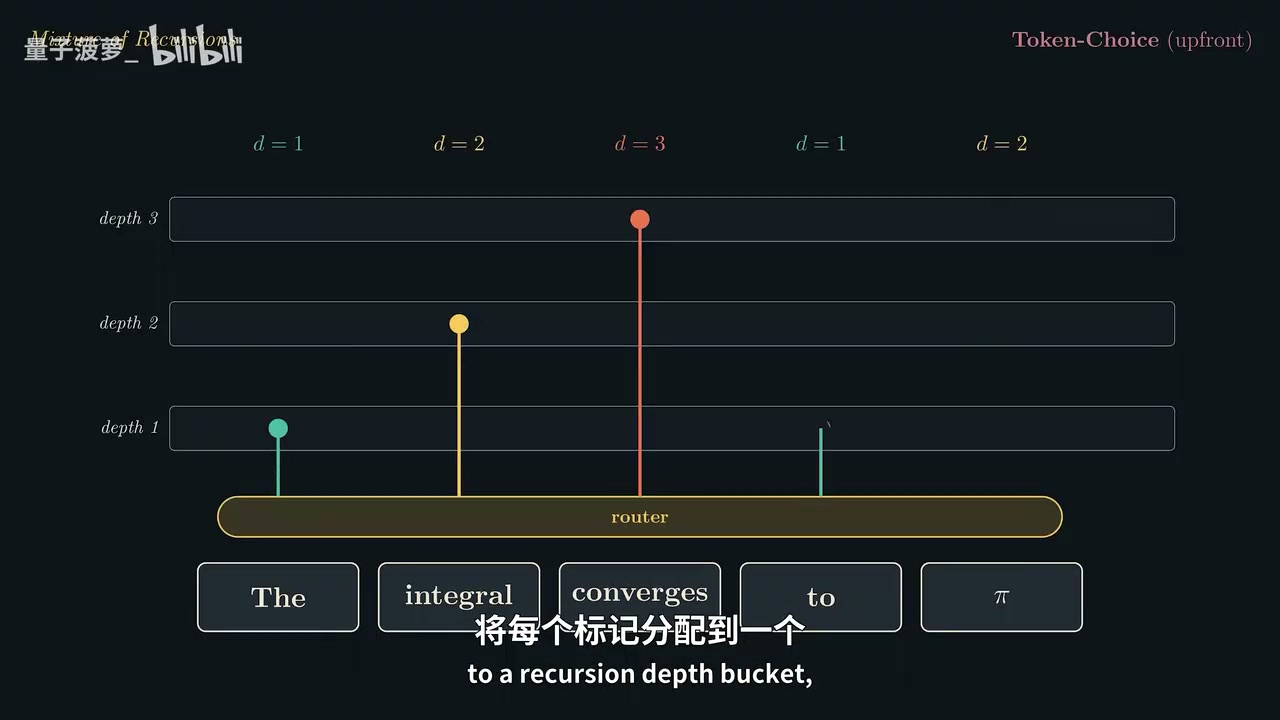
\includegraphics[width=0.82\linewidth,height=0.36\textheight,keepaspectratio]{figures/fig_11_token_choice_routing.jpg}
  \caption{Token-choice 预分配路由：每个 token 在循环开始前被分到递归深度桶，执行路径规整，代价是依赖早期难度判断。\protect\footnotemark}
  \label{fig:mor-token-choice-routing}
\end{figure}
\footnotetext{视频画面时间区间：00:11:42--00:12:00。}

这种方式的工程优点很清楚：路径从一开始就固定，调度更容易，批处理更整齐。主要风险也同样清楚：如果初始状态还没有足够信息判断 token 难度，早期误判后面很难纠正。视频在 00:11:53--00:12:00 正是这样描述它的限制。

\subsection{Expert-choice：递归过程中的逐步退出}

第二种方式是 expert-choice routing（逐步路由）。视频在 00:12:00--00:12:20 说明，模型在每次迭代时可以选择继续或退出。图中 token 会在不同深度处出现 exit 决策，路径随递归过程逐步确定。

先用白话解释公式：第 \(i\) 个 token 在第 \(t\) 次递归后，路由器根据当前状态 \(h_{i,t}\) 判断继续还是退出。因为 \(h_{i,t}\) 已经包含前几轮更新后的信息，这种判断通常比只看初始状态更灵活。

\[
a_{i,t}=g_\phi(h_{i,t}),\qquad a_{i,t}\in\{\mathrm{continue},\mathrm{exit}\}
\]

符号说明：
\begin{itemize}
  \item \(a_{i,t}\)：第 \(i\) 个 token 在第 \(t\) 步的路由动作。
  \item \(h_{i,t}\)：第 \(i\) 个 token 在第 \(t\) 次递归后的隐藏状态。
  \item \(g_\phi\)：逐步路由器函数。
  \item \(\mathrm{continue}\)：继续进入下一轮递归。
  \item \(\mathrm{exit}\)：退出递归，停止为该 token 分配后续循环计算。
\end{itemize}

\begin{figure}[htbp]
  \centering
  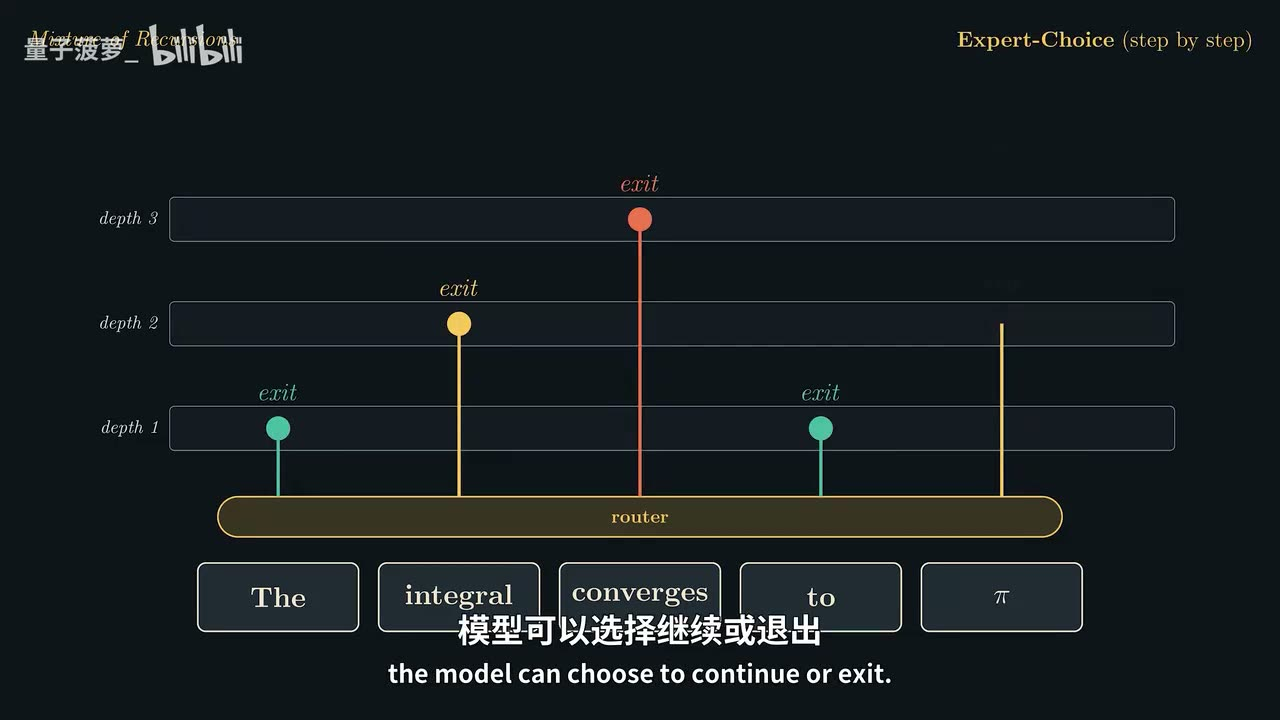
\includegraphics[width=0.82\linewidth,height=0.36\textheight,keepaspectratio]{figures/fig_12_expert_choice_routing.jpg}
  \caption{Expert-choice 逐步路由：token 可在每轮递归后选择继续或退出，适应性更强，训练与调度也更复杂。\protect\footnotemark}
  \label{fig:mor-expert-choice-routing}
\end{figure}
\footnotetext{视频画面时间区间：00:12:05--00:12:20。}

逐步路由的优势来自“边计算边判断”。当模型完成一两轮更新后，某些 token 的表示已经足够稳定，继续递归收益很低；另一些 token 仍处在关系整合阶段，需要更多更新。这个机制更贴近按需计算，但每一步都要做路由决策，也会让训练目标、负载均衡、梯度稳定和批处理效率变得更难处理。

\subsection{自适应计算量：MoR 的节省从哪里来}

MoR 的成本直觉可以用一条公式压缩：每个 token 只支付自己实际使用的递归深度。若第 \(i\) 个 token 的深度是 \(d_i\)，总计算量随所有 \(d_i\) 之和增长。

\[
C_{\mathrm{MoR}}\propto \sum_{i=1}^{n}d_i,\qquad C_{\mathrm{MoR}}\le C_{\mathrm{fixed}}\ \mathrm{when}\ d_i\le R
\]

符号说明：
\begin{itemize}
  \item \(C_{\mathrm{MoR}}\)：MoR 的近似计算量。
  \item \(n\)：序列中的 token 数。
  \item \(d_i\)：第 \(i\) 个 token 实际使用的递归深度。
  \item \(R\)：固定递归方案中的最大递归步数。
  \item \(C_{\mathrm{fixed}}\)：所有 token 都运行 \(R\) 步时的近似计算量。
\end{itemize}

这条公式的教学意义是：MoR 的收益不来自“循环本身免费”，而来自把递归步数集中给更需要的 token。若所有 token 最后都跑满 \(R\)，MoR 没有节省；若大量 token 早退，节省才会出现。

\begin{knowledgebox}{路由器直觉}
可以把 MoR 想成考场里的分题时间管理。简单题一眼能做完，就不该占用整张卷子的时间；难题需要多轮推导，可以拿更多时间。固定递归像每道题强制写满三页草稿，MoR 则把草稿纸按题目难度分配。
\end{knowledgebox}

\subsection{视频给出的路由对比与必要谨慎}

视频在 00:12:20--00:12:48 给出的对比是：在相同的三递归设置下，逐步版本被称为 expert-choice routing，平均少样本准确率约为 \(42.6\%\)；前期分配版本被称为 token-choice routing，约为 \(40\%\)。讲义应把这写成视频给出的对比，而非普遍定律。原因有三点。

第一，字幕和口播可能简化了论文术语，routing 名称与具体实现需要最终由画面或原论文确认。第二，\(42.6\%\) 与 \(40\%\) 是特定设置下的视频叙述，不能推出 expert-choice 在所有任务、模型规模和递归深度下都更好。第三，token-choice 的理论整洁性和工程调度优势仍然存在，数值落后可能来自早期难度预测过难、训练配置、任务类型或评价设置。

\begin{warningbox}{指标解读边界}
本章沿用视频画面和口播中的 routing 名称：token-choice 表示循环前预分配，expert-choice 表示逐步继续或退出。数值部分应写作“视频给出的对比是 expert-choice 约 \(42.6\%\)，token-choice 约 \(40\%\)”；在最终整合前，若要写成论文级结论，需要核验原论文表格与指标定义。
\end{warningbox}

\subsection{本章小结}

本章把循环模型的效率问题从“是否能多想几轮”推进到“哪些 token 值得多想”。读者应带走三点：第一，固定递归会让简单 token 和复杂 token 支付同样计算成本；第二，token-choice 在循环前预分配深度，执行规整但依赖早期判断；第三，expert-choice 在递归过程中逐步决定继续或退出，更灵活也更难训练。视频给出的 \(42.6\%\) 与 \(40\%\) 对比只能作为该视频语境下的指标线索，不能被扩展成无条件的路由优劣结论。下一章需要继续处理真实推理系统里的 KV cache，因为节省参数和递归步数之后，内存带宽仍会追上来。

% END INLINE section_06.tex

% BEGIN INLINE section_07.tex
\section{KV cache：递归节省参数后，内存带宽仍会追上来}
\label{sec:kv-cache}

本章结论很直接：循环 Transformer（Loop Transformer）通过共享参数减少了模型权重，却不会自动减少推理时的内存读写。自回归解码中的 KV 缓存（KV cache, key-value cache）保存的是每层、每个 token 的注意力键和值；一旦递归深度也需要各自的注意力状态，内存带宽会把架构层面的节省重新拉回系统成本表里。

\begin{importantbox}{本章主张}
“参数少”只说明模型权重更紧凑；“运行时更省”还要看每步推理搬运了多少激活、KV 张量和缓存状态。Loop Transformer 若按朴素方式为每个递归深度保留 KV，部署瓶颈很可能从参数容量转移到内存带宽。
\end{importantbox}

\subsection{为什么共享参数没有自动消除缓存压力}

标准 Transformer 在生成下一个 token 时，会把历史 token 在各层 attention 中产生的 key 和 value 存下来。这样后续解码无需重新计算整个前缀，代价是缓存规模随上下文长度、层数、头数和 hidden size 增长。视频在 00:12:59--00:13:20 强调的核心点是：循环模型即使复用同一组参数，仍可能在不同递归深度上产生不同的隐藏状态；只要这些状态要参与 attention，就需要相应的 KV。

\begin{knowledgebox}{KV cache 直觉}
KV 缓存可以类比成图书馆的索引卡。权重参数像馆员的工作规则，KV 缓存像已经为当前读者整理好的索引。馆员规则可以复用，索引卡仍会随着读者已经读过的页数、查询轮数和索引版本增长。
\end{knowledgebox}

\begin{figure}[htbp]
  \centering
  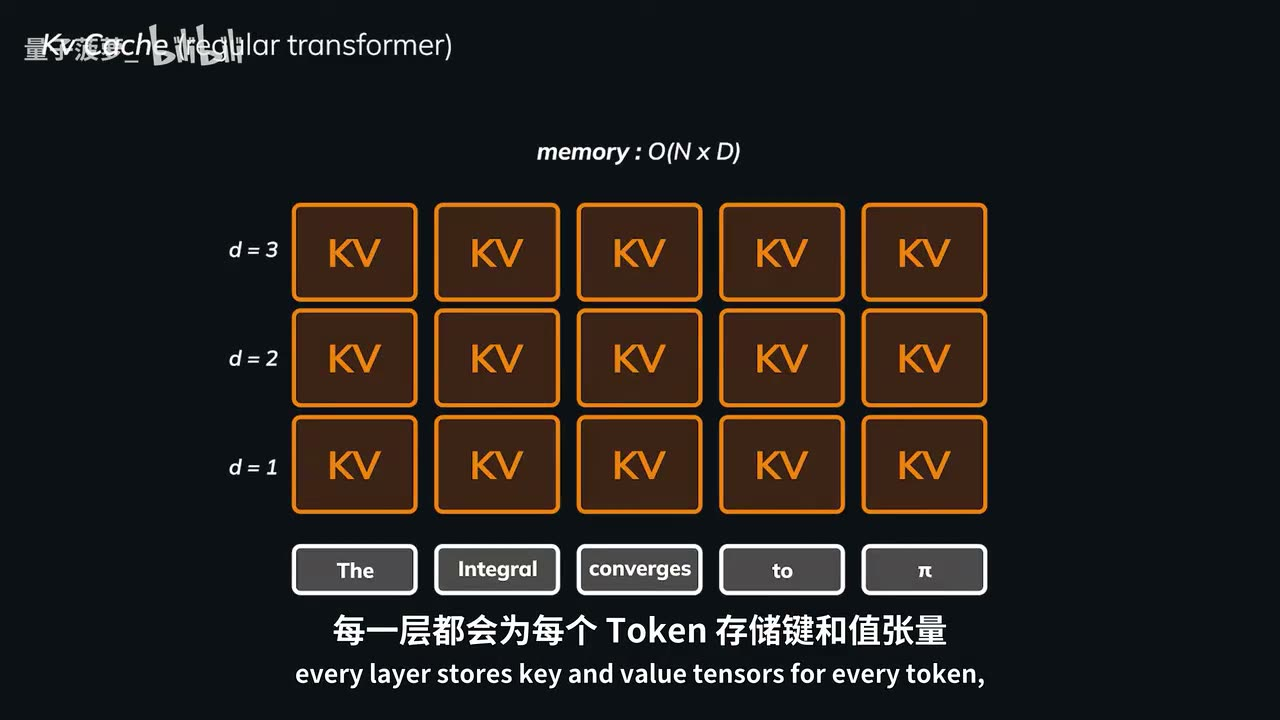
\includegraphics[width=0.82\linewidth,height=0.36\textheight,keepaspectratio]{figures/fig_13_recursive_kv_cache.jpg}
  \caption{朴素递归模型的 KV cache 压力：共享参数减少了权重副本，递归深度仍可能引入多份 KV 状态。\protect\footnotemark}
  \label{fig:recursive-kv-cache}
\end{figure}
\footnotetext{视频画面时间区间：00:12:59--00:13:20。}

\subsection{朴素递归缓存的放大}

先用一句白话说明公式要表达的东西：如果每个 token 在每个递归深度都留下独立 KV，那么缓存大小会同时随上下文 token 数和递归步数增长。递归深度 \(R\) 省下的是同一模块的参数副本，未必省下每一步产生的状态副本。

$
M_{\mathrm{naive}}\propto nR d_{\mathrm{model}}
$

\begin{itemize}
  \item \(M_{\mathrm{naive}}\)：朴素递归 KV 缓存的近似内存量。
  \item \(n\)：当前上下文中的 token 数。
  \item \(R\)：最大递归深度，也就是共享模块最多被重复应用的次数。
  \item \(d_{\mathrm{model}}\)：每个 token 表示的模型维度；真实系统还会乘上层数、注意力头数、K/V 两份张量和数值精度字节数。
  \item \(\propto\)：表示只看主导比例关系，省略实现相关常数。
\end{itemize}

这个式子的工程含义很硬：循环架构省参数，缓存系统仍可能要为 \(n\times R\) 个状态服务。在长上下文解码中，GPU 计算单元经常等待显存读写；此时 FLOPs 账面节省无法直接转化成吞吐提升。

\begin{warningbox}{部署评估提醒}
评估循环模型时，单看参数量和理论计算量容易误判。真实服务还要测每 token 延迟、批处理吞吐、显存峰值、KV 读写带宽和缓存命中形态。递归让计算更紧凑，也可能让状态管理更复杂。
\end{warningbox}

\subsection{递归感知缓存：只为活跃 token 付费}

递归感知缓存（recursion-aware cache）的思路是让缓存跟着 MoR 的自适应递归走：已经提前退出的 token 停止产生更深递归的 KV，仍在思考的 token 继续保留当前步所需的 key/value。这样，越往深处走，活跃 token 数 \(n_t\) 越少，缓存和 attention 计算随之收缩。

这条公式表达的是“每一层递归只为仍活跃的 token 保存状态”，所以总内存由各递归步的活跃 token 数累加决定。

$
M_{\mathrm{aware}}\propto \sum_{t=1}^{R} n_t d_{\mathrm{model}},\qquad n_{t+1}\le n_t
$

\begin{itemize}
  \item \(M_{\mathrm{aware}}\)：递归感知缓存的近似内存量。
  \item \(t\)：递归步编号。
  \item \(R\)：最大递归深度。
  \item \(n_t\)：第 \(t\) 次递归仍处于活跃状态的 token 数。
  \item \(d_{\mathrm{model}}\)：每个 token 的表示维度。
  \item \(n_{t+1}\le n_t\)：表示 token 可以提前退出，所以后续递归的活跃集合通常不增大。
\end{itemize}

递归感知缓存的优势来自“新鲜”：每一步都使用当前递归步更新后的表示来生成 KV。它更符合模型正在逐步修正隐藏状态的事实，质量通常更稳。代价也清楚：仍活跃的 token 会在多个深度保留新版本 KV，显存占用和缓存写入量高于最激进的共享方案。

\subsection{递归 KV 共享：省内存的代价是表示变旧}

递归 KV 共享（recursive KV sharing）进一步压缩缓存：模型在较早递归步生成 KV，后续递归复用这份缓存，减少跨递归深度复制。直觉上，它像拍下第一轮草稿的索引快照，后面多轮修改时继续查这份快照。这样显存更省，隐藏状态的最新变化也更难完整反映到 attention 读写中。

用最简化形式表示，递归共享把深度维度从缓存主项中拿掉，使缓存近似随 token 数增长。

$
M_{\mathrm{share}}\propto n d_{\mathrm{model}}
$

\begin{itemize}
  \item \(M_{\mathrm{share}}\)：递归 KV 共享的近似内存量。
  \item \(n\)：上下文 token 数。
  \item \(d_{\mathrm{model}}\)：每个 token 表示的模型维度。
  \item 省略的常数：层数、头数、K/V 两份张量、数值精度和具体缓存布局。
\end{itemize}

\begin{figure}[htbp]
  \centering
  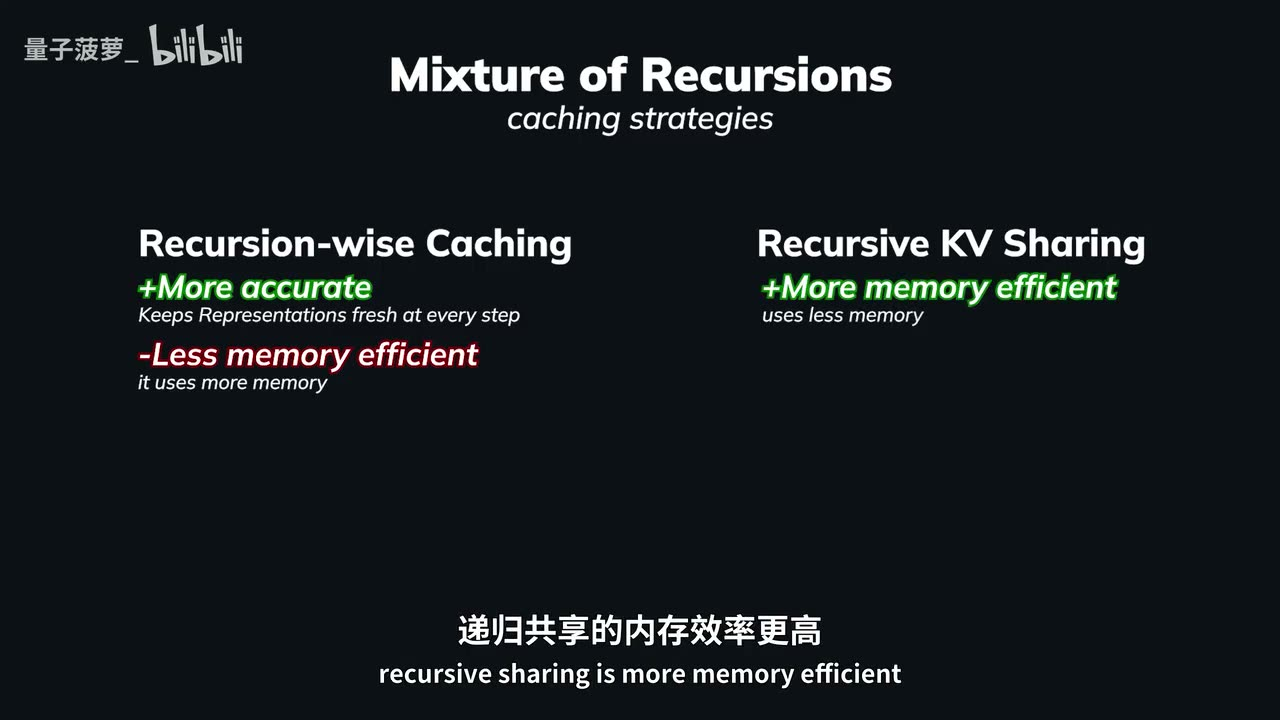
\includegraphics[width=0.82\linewidth,height=0.36\textheight,keepaspectratio]{figures/fig_14_mor_cache_tradeoff.jpg}
  \caption{MoR 缓存策略的权衡：递归感知缓存保持表示新鲜，递归 KV 共享更节省内存。\protect\footnotemark}
  \label{fig:mor-cache-tradeoff}
\end{figure}
\footnotetext{视频画面时间区间：00:14:15--00:14:25。}

因此，缓存策略的核心取舍是内存效率和表示新鲜度。递归感知缓存更适合质量优先或活跃 token 很快减少的场景；递归 KV 共享更适合显存紧张、带宽敏感、可以接受少量质量折损的场景。视频里提到这些权衡在论文实验中可控，并且和自适应路由结合后有机会优于朴素递归模型与标准 Transformer；这个判断仍需要在具体任务、上下文长度和服务批量下重新测量。

\subsection{本章小结}

KV cache 把 Loop Transformer 从“架构参数问题”带回“推理系统问题”。本章应带走三点：

\begin{itemize}
  \item 共享参数降低权重存储，不保证降低每步 attention 状态的内存流量。
  \item 朴素递归缓存的压力近似随 \(nR\) 增长，长上下文会把显存和带宽瓶颈放大。
  \item 递归感知缓存用更多新鲜 KV 换质量，递归 KV 共享用较旧 KV 换内存效率；两者都属于工程权衡，需要用真实延迟、吞吐和质量指标一起评估。
\end{itemize}

% END INLINE section_07.tex

% BEGIN INLINE section_08.tex
\section{边界判断：表达能力、真实深度、监督信号与部署位置}
\label{sec:limits-deployment}

本章结论是全文的冷水区：Loop Transformer 的研究价值真实存在，优势来自“用计算换有效深度，用共享参数换紧凑模型”；它尚未被证明可以作为标准 Transformer 或思维链（Chain-of-Thought, CoT）的通用替代方案。它能否成为实用路线，取决于表达能力、真实深度、监督信号、KV cache 和部署约束能否同时过关。

\begin{importantbox}{本章主张}
Loop Transformer 适合被理解为一种带强归纳偏置的递归计算方案。它把模型推向“反复更新同一份隐藏表示”的路线；标准 Transformer 的深层堆栈则给每一层独立参数和独立变换空间。二者的系统价值要按任务、内存、延迟和训练信号共同判断。
\end{importantbox}

\subsection{表达能力：共享权重是一种约束}

表达能力（expressiveness）指模型函数族能表示多复杂的输入输出关系。视频在 00:14:48--00:15:17 提醒读者：拥有独立层的更深或更宽模型通常有更大的自由度；如果内存和参数预算宽松，标准 Transformer 可以通过增加层数、宽度和参数量获得更低损失，并避开递归 KV 管理的复杂性。

用公式先表达结构差异。独立深层堆栈把多个不同变换串起来；递归深度把同一个共享变换反复应用。这个公式只说明架构约束，不能直接推出哪个模型在所有任务上更强。

$
h_L = F_L\circ F_{L-1}\circ \cdots \circ F_1(x),\qquad
h_R = \underbrace{F_\theta\circ F_\theta\circ \cdots \circ F_\theta}_{R\ \mathrm{steps}}(x)
$

\begin{itemize}
  \item \(x\)：输入 token 或输入隐藏表示。
  \item \(h_L\)：经过 \(L\) 个独立层后的表示。
  \item \(F_1,\ldots,F_L\)：每层各自拥有参数的 Transformer 变换。
  \item \(h_R\)：经过 \(R\) 次递归后的表示。
  \item \(F_\theta\)：参数 \(\theta\) 共享的循环模块。
  \item \(\circ\)：函数复合，表示前一个变换的输出进入下一个变换。
\end{itemize}

\begin{figure}[htbp]
  \centering
  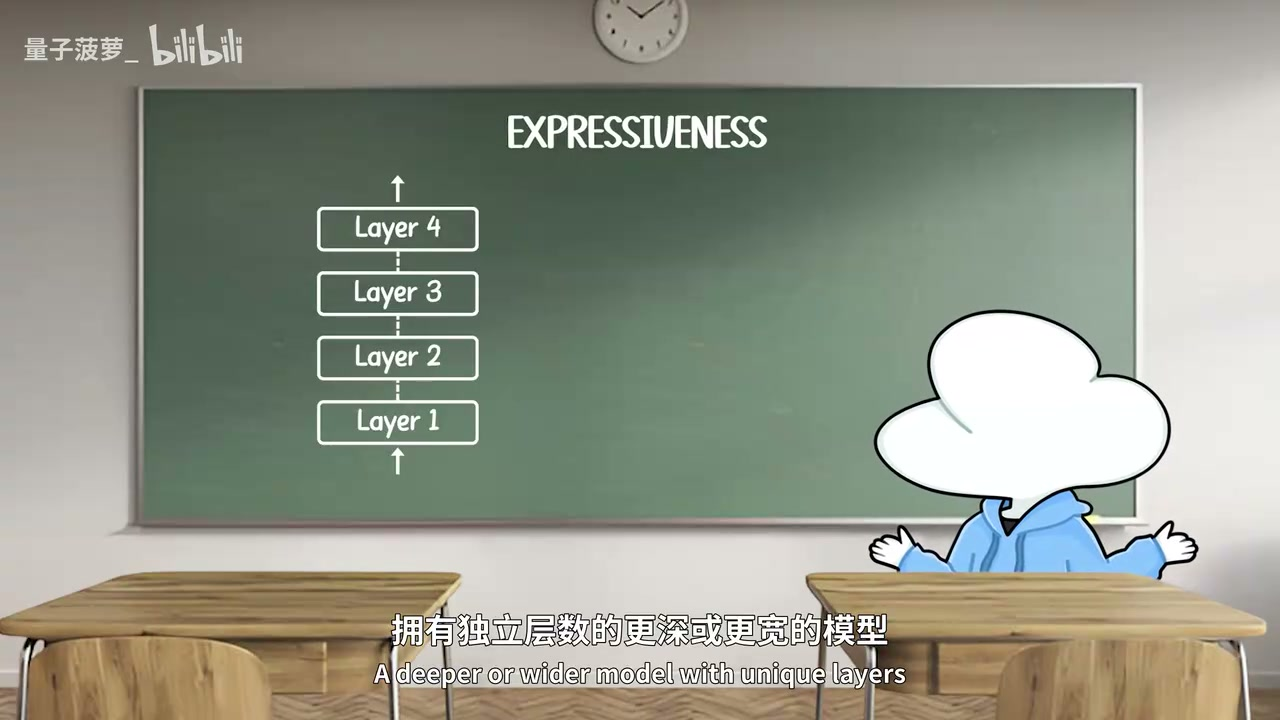
\includegraphics[width=0.82\linewidth,height=0.36\textheight,keepaspectratio]{figures/fig_15_expressiveness_comparison.jpg}
  \caption{表达能力边界：独立深层或更宽模型拥有更大的参数自由度，共享递归块是一种更紧凑的受约束选择。\protect\footnotemark}
  \label{fig:expressiveness-comparison}
\end{figure}
\footnotetext{视频画面时间区间：00:14:48--00:15:17。}

这里有一个容易漏掉的背景：扩展定律（scaling laws）的历史经验更偏向增加参数量和数据量。重复利用计算想要成为主路线，需要证明它在同等系统预算下带来更高质量、更低成本或更好的可部署性。

\subsection{真实深度与递归深度}

真实深度（real depth）意味着每一层都可以学习自己的变换；递归深度（recurrent depth）意味着同一函数在不同状态上重复执行。前者给模型显式的分层归纳偏置，后者依赖隐藏状态的演化让同一共享模块在早期、中期、后期表现出不同功能。

上一章之前的机制分析给了积极信号：共享块在不同递归阶段可能承担粗略表示、关系整合、答案收敛等角色。边界也同样明确：这种阶段化行为需要模型自己学出来；独立深层堆栈把“每一步可以不同”直接写进参数结构里。

\begin{figure}[htbp]
  \centering
  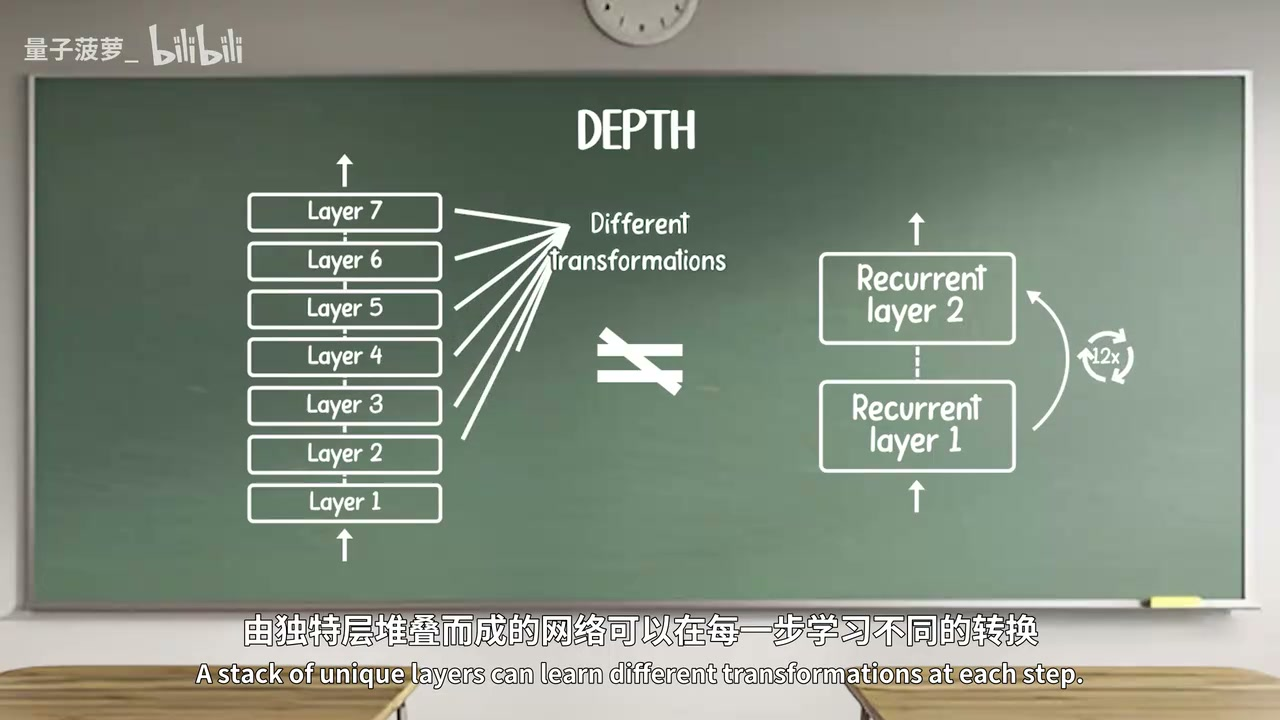
\includegraphics[width=0.82\linewidth,height=0.36\textheight,keepaspectratio]{figures/fig_16_depth_comparison.jpg}
  \caption{真实深度与递归深度的差异：独立层提供不同变换，循环层复用同一函数并依赖状态演化产生阶段差异。\protect\footnotemark}
  \label{fig:depth-comparison}
\end{figure}
\footnotetext{视频画面时间区间：00:15:31--00:16:10。}

\begin{warningbox}{深度误读}
把“循环次数更多”直接读成“模型等价于更深的 Transformer”会误导判断。递归深度增加了计算步数，也增加了同一函数反复作用的机会；真实深度增加的是可学习变换的种类和参数自由度。
\end{warningbox}

\subsection{推理收益的证据边界}

视频对多跳推理和深度外推保持了谨慎态度。受控基准中的多跳结果很有价值，因为它们说明递归深度可能形成可复用的计算过程；这些结果距离大规模真实任务还有距离。真实任务包含长上下文噪声、开放域知识、工具调用、格式约束、多轮交互和分布漂移，循环深度在这些条件下能否稳定贡献收益，需要更多实验。

这也是“房间里的大问题”：如果计算和内存允许，直接加深或加宽标准 Transformer 可能更简单；如果参数预算很紧，Loop Transformer 才更容易显出独特价值。研究判断要追问的是边际收益：多花一次递归步，和多加一层独立层、多生成若干 CoT token、增大批量或优化 KV cache 相比，哪个更划算。

\subsection{CoT 的监督信号优势}

CoT 的工程价值除了推理时多写 token，还在于它留下了显式文本轨迹。这些轨迹可以被人工筛选，可以用于监督学习，可以作为强化学习的过程信号，也可以被学生模型模仿。换句话说，CoT 把“思考过程”变成可存储、可审查、可训练的数据。

Loop Transformer 的隐藏状态递归更紧凑，也更难监督。中间计算藏在连续向量里，没有自然语言标签告诉模型第一步、第二步、第三步应如何组织。训练只能更多依赖最终目标，或者依赖额外的探针、辅助损失、蒸馏教师和轨迹约束。这些方案有研究空间，也会增加训练设计难度。

\begin{figure}[htbp]
  \centering
  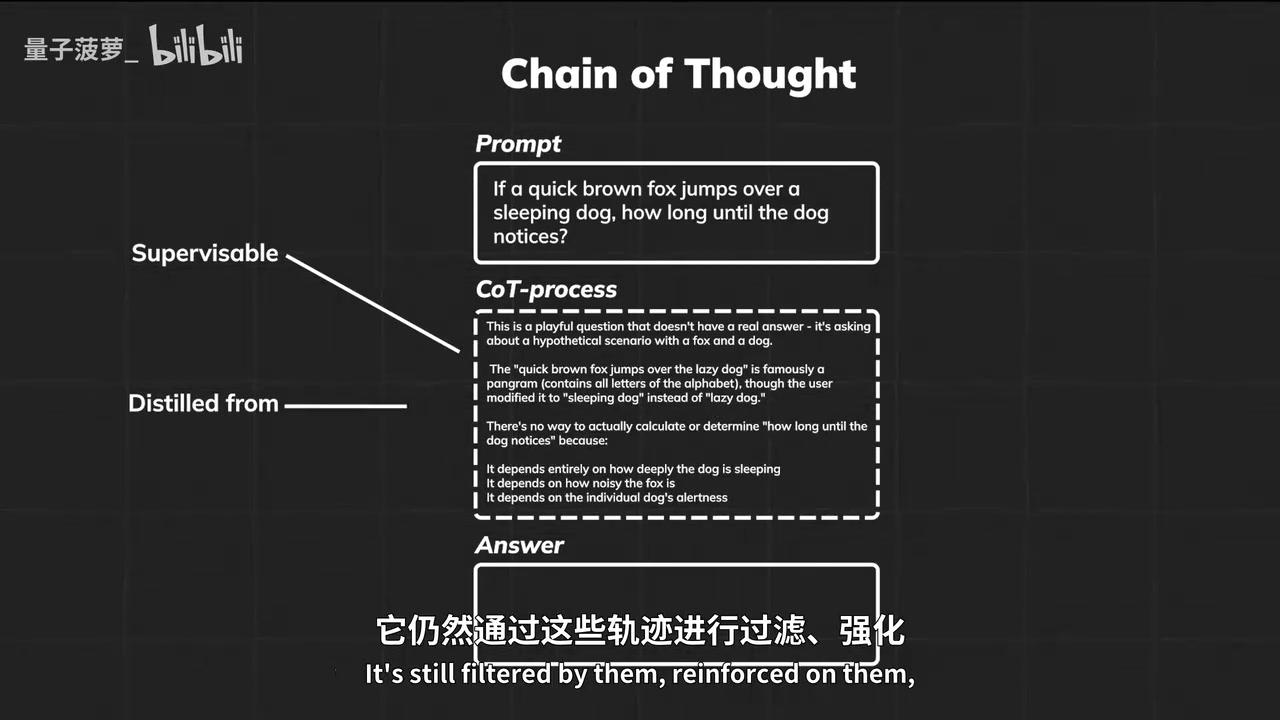
\includegraphics[width=0.82\linewidth,height=0.36\textheight,keepaspectratio]{figures/fig_17_cot_vs_looped_model.jpg}
  \caption{CoT 的显式轨迹优势：文本中间步骤便于监督、筛选、强化和蒸馏；隐藏状态递归缺少天然中间标签。\protect\footnotemark}
  \label{fig:cot-vs-looped-model}
\end{figure}
\footnotetext{视频画面时间区间：00:16:34--00:17:23。}

\begin{knowledgebox}{监督信号类比}
可以把 CoT 轨迹理解为学生写在草稿纸上的解题步骤。教师能批改每一步，挑出好草稿，训练另一个学生模仿。隐藏状态递归更像学生在脑内默算，答案也许正确，教师很难知道中间哪一步值得奖励或修正。
\end{knowledgebox}

\subsection{可能的部署位置}

视频给出的潜在落点集中在资源受限或同参数竞争场景：合成数据生成（synthetic data generation）、蒸馏（distillation）、边缘部署（edge deployment）、移动设备小模型，以及 CoT 成本过高或同参数模型能力不足的场景。这里的关键词是“约束”。当参数容量是主要瓶颈，递归计算能把有限参数重复使用；当服务瓶颈是延迟和吞吐，重复模块的序列化成本会变得刺眼。

\begin{figure}[htbp]
  \centering
  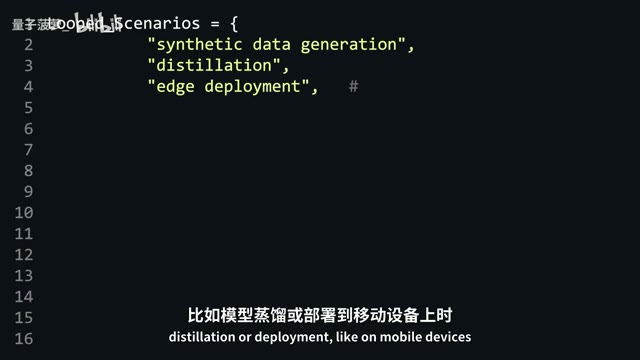
\includegraphics[width=0.72\linewidth,height=0.30\textheight,keepaspectratio]{figures/fig_18_application_scenarios.jpg}
  \caption{潜在应用场景：合成数据生成、蒸馏和边缘部署更容易体现共享参数与递归计算的价值。\protect\footnotemark}
  \label{fig:application-scenarios}
\end{figure}
\footnotetext{视频画面时间区间：00:17:23--00:17:40。}

实践者应把 Loop Transformer 放进系统指标里评估：同等参数量下质量是否提升，同等延迟下吞吐是否下降，长上下文 KV cache 是否可控，路由器是否稳定，训练数据中是否存在足够的过程信号。少看单点指标，多看质量、成本和部署约束的共同边界。

\subsection{本章小结}

本章形成三点判断：

\begin{itemize}
  \item Loop Transformer 的优势来自用计算换有效深度，用共享参数换紧凑模型；它的代价是表达能力约束、递归状态管理和更难监督的内部过程。
  \item 它的研究价值取决于稳定性、自适应路由、KV cache 和训练监督能否一起成立；只解决其中一项，仍不足以支撑大规模默认替代路径。
  \item 它近期更像特定约束下的工程与研究选项，尤其适合小模型、边缘部署、蒸馏和同参数量竞争；在大规模 LLM 服务中，标准 Transformer 与 CoT 仍拥有强大的训练、扩展和部署惯性。
\end{itemize}

% END INLINE section_08.tex

% BEGIN INLINE section_09.tex
\section{总结与延伸}
\label{sec:synthesis}

全篇可以压缩成一个判断：Loop Transformer 把思维链的外部文本迭代，改写为隐藏状态中的内部递归；这条路线有清楚的技术吸引力，也有硬边界。它让模型用共享模块反复更新表示，可能在同等参数量下获得更深的有效计算；它也把稳定性、自适应计算、KV cache、监督信号和部署成本集中成一组必须同时解决的问题。Loop Transformer 尚未被证明可以通用替代标准 Transformer 或 CoT。

\subsection{从 CoT 到内部递归的主线}

视频的技术主线从一个朴素问题开始：为什么模型通过生成更多 token 能推理得更好？答案是测试时计算（test-time compute）给模型提供了迭代空间。CoT 把中间步骤写成文本，模型再读回这些文本，继续更新状态。这个流程有效，因为它制造了可见的推理轨迹；它也昂贵，因为每轮都要经历文本生成、上下文追加、重新嵌入和再次条件化。

Loop Transformer 的核心改动是把这条外部轨迹移回隐藏状态。共享的 Transformer 模块反复作用于残差流，让模型在连续向量空间里修正表示。多跳推理、三阶段泛化、PCA 轨迹、固定点和周期轨迹给了研究线索：递归可能形成结构化内部过程，且同一共享块在不同递归阶段可能承担不同功能。

随后，MoR（Mixture-of-Recursions）把固定递归步数改造成 token 级自适应计算：简单 token 提前退出，复杂 token 获得更多递归。KV cache 章节把讨论拉回系统现实：共享参数无法自动减少运行时状态，递归感知缓存和递归 KV 共享分别在表示新鲜度与内存效率之间取舍。

\begin{importantbox}{总判断}
最稳妥的整体判断是：Loop Transformer 是一条把参数共享、递归深度、动态系统稳定性、自适应计算和推理系统缓存绑定在一起的研究路线。它的亮点在“紧凑模型如何获得更多内部计算”，它的风险在“内部计算如何稳定、监督和高效部署”。
\end{importantbox}

\subsection{开放问题}

以下问题决定这条路线能走多远：

\begin{itemize}
  \item 隐藏状态递归如何监督：缺少文本中间步骤后，模型如何获得过程级训练信号，怎样避免只靠最终答案学习出脆弱策略。
  \item 路由器如何稳定训练：token 何时继续、何时退出，既影响质量，也影响计算图和负载均衡。
  \item KV cache 策略怎样影响真实吞吐：递归感知缓存、递归 KV 共享和朴素缓存的差异需要在长上下文、批处理和真实硬件上测量。
  \item 受控基准能否迁移到真实任务：多跳推理和深度外推是有力线索，开放域推理、工具调用、多轮对话和高噪声上下文仍需要独立验证。
  \item 递归深度怎样选择：固定最大深度、动态早停、置信度门控和预算约束会直接改变延迟、质量与能耗。
  \item 可解释证据如何建立：PCA 轨迹能显示状态形状，仍需要更多机制分析证明模型内部递归对应可靠推理步骤。
\end{itemize}

\subsection{实践评估建议}

实践者不应把 Loop Transformer 当成架构口号来评估。更可操作的做法是把它放进预算表：

\begin{itemize}
  \item 若主要限制是参数容量、设备显存或模型下发体积，可以重点关注递归深度是否在同参数量下提升质量。
  \item 若主要限制是服务延迟和吞吐，需要谨慎评估重复模块带来的序列化成本，并测量每 token 延迟、批处理吞吐和显存带宽。
  \item 若任务依赖可审查的推理过程，CoT 的显式轨迹仍有训练和审核优势；隐藏递归需要额外探针、辅助损失或蒸馏设计。
  \item 若任务是合成数据生成、蒸馏或边缘部署，可以把 Loop Transformer 作为候选方案，与小型标准 Transformer、短 CoT、早停解码和缓存优化一起比较。
  \item 若实验只报告受控多跳结果，应继续要求长上下文、真实分布、不同批量、不同硬件和失败案例分析。
\end{itemize}

\subsection{可带走的判断清单}

\begin{enumerate}
  \item CoT 的本质价值是外部化迭代：它给模型更多测试时计算，也给训练者可见轨迹。
  \item Loop Transformer 的本质价值是内部化迭代：它让隐藏状态在共享模块中反复更新，用递归深度换有效计算。
  \item 动态系统稳定性是循环架构的地基：递归会放大偏差，也可能形成固定点、周期和阶段化推理。
  \item MoR 的价值在按需计算：简单 token 少走几步，复杂 token 多走几步，收益取决于路由判断是否可靠。
  \item KV cache 是部署硬约束：参数共享没有自动消除缓存读写，缓存策略会直接决定真实吞吐。
  \item 边界判断必须保守：Loop Transformer 是值得关注的研究方向，尚未成为大规模通用 LLM 架构的默认替代路线。
\end{enumerate}

\subsection{来源边界说明}

本讲义的技术主线来自视频字幕、元数据和已抽取画面候选区间；00:18:05 之后的视频内容主要转入评论互动、课程推广、鸣谢和社交媒体提醒，正文已将这些频道推广信息排除在技术讲解之外。涉及论文命名、具体数值和方法优劣时，本文保持视频范围内的审慎表述；后续若要作为研究引用，应回到原论文和公开实验设置继续核验。

\subsection{拓展阅读}

以下资料用于把视频讲解中的关键论文线索和原始研究入口对应起来。阅读时应区分三层证据：视频讲解负责建立直觉，论文负责给出实验设置和方法细节，工程落地还需要在目标硬件、目标任务和目标延迟预算中重新测量。

\begingroup
\small
Harsh Kohli 等，\href{https://arxiv.org/abs/2604.07822}{\emph{Loop, Think, \& Generalize: Implicit Reasoning in Recurrent-Depth Transformers}}，arXiv:2604.07822，2026-04-09；Hugh Blayney 等，\href{https://arxiv.org/abs/2604.11791}{\emph{A Mechanistic Analysis of Looped Reasoning Language Models}}，arXiv:2604.11791，2026-04-13；Hayden Prairie 等，\href{https://arxiv.org/abs/2604.12946}{\emph{Parcae: Scaling Laws For Stable Looped Language Models}}，arXiv:2604.12946，2026-04-14；Sangmin Bae 等，\href{https://arxiv.org/abs/2507.10524}{\emph{Mixture-of-Recursions: Learning Dynamic Recursive Depths for Adaptive Token-Level Computation}}，arXiv:2507.10524，2025-07-14。
\par
\endgroup

\subsection{术语速记}

最后把容易混在一起的术语压缩成一张复盘表。它的作用是帮助读者回到正文时快速定位：哪些概念属于推理方式，哪些概念属于模型结构，哪些概念属于系统部署。

\begin{itemize}
  \item CoT：把中间步骤写成文本 token，优势是轨迹可见、训练信号清楚，代价是上下文和解码成本增加。
  \item 递归深度：同一共享模块被重复调用的次数，作用近似给模型增加测试时计算预算。
  \item 残差流：隐藏状态持续传递的主通道，循环模型的内部“草稿纸”主要在这里被反复改写。
  \item 固定点与周期：动态系统的稳定结构，提示递归状态可能在收敛或有规律地往复。
  \item MoR：让不同 token 使用不同递归步数，用路由器把计算预算分给更复杂的位置。
  \item KV cache：部署时的内存和带宽约束；参数共享节省的是权重存储，缓存策略决定运行时吞吐。
\end{itemize}

% END INLINE section_09.tex

\end{document}


